\documentclass[../main.tex]{subfiles}

%\graphicspath{{\subfix{../images/}}}

\begin{document}
\subsection{Definitions}
\subsubsection{Group}
\begin{itemize}
\item closure: $a,b\in G \rightarrow a\circ b \in G$
\item associativity: $a\circ b)\circ c=a\circ(b\circ c)$
\item identity: $\exists e\in G$ s.t. $a\circ e=e\circ a = a$
\item inverse: $\forall a\in G,\; \exists a^{-1}\in G$ s.t. $a\circ a^{-1}=a^{-1}\circ a=e$
\end{itemize}

\subsubsection{Lie Group}
Continuous group

\subsubsection{Group Representation}
\begin{itemize}
\item $D_R:G\rightarrow \text{GL}(n)$ s.t. $D_R(a)D_R(b)=a\circ b$
\item $D(e)=1_{n\times n}$
\item $D(a^{-1})=D(a)^{-1}$
\end{itemize}

\subsubsection{Lie Algebra Representation}
\begin{itemize}
\item $\pi:\mathfrak{g} \rightarrow \text{Mat}(n)$ s.t. $\pi([A,B])=[\pi(A),\pi(B)]$
\end{itemize}

\subsubsection{Lie Algebra vs Lie Group}
Lie group element $a(\theta)$, representation of group element $D_R(a(\theta))$, representation of Lie algebra generator $\pi_R(A^\mu)$
\begin{align}
D_R(a(\theta))&=e^{i\theta_\mu\pi_R(A^\mu)}\\
\pi_R(A^\mu)&=-i\left.\frac{\partial D_R}{\partial\theta_\mu}\right|_{\theta=0}
\end{align}

\subsubsection{Matrix Exponentials}
\begin{align}
e^X&=\sum_{n=0}\frac{1}{n!}X^n\\
\text{det}\;e^X&=e^{\text{tr} X} \\
\left(e^X\right)^{-1}&=e^{-X}\\
e^Xe^Y&=e^{X+Y+\frac{1}{2}[X,Y]+\frac{1}{12}[X,[X,Y]]-\frac{1}{12}[Y,[X,Y]]+...}
\end{align}


\subsubsection{Irreducible representation}
$ D_{R_1} \oplus D_{R_2} \neq D_R$

\subsubsection{Casimir element/operator}
Object (element of the center of the universal enveloping algebra of a Lie algebra) that commutes with all generators of the Lie algebra

\subsection{Representation facts you should know as a physicist}



\subsection{SU(2) and Quantum mechanics of spin 1/2}
\begin{itemize}
\item Definitions I: Pauli matrices
\begin{align}
\sigma_1=\left(\begin{matrix}
0 & 1\\
1 & 0
\end{matrix}
\right),\qquad
\sigma_2=\left(\begin{matrix}
0 & -i\\
i & 0
\end{matrix}
\right),\qquad
\sigma_3=\left(\begin{matrix}
1 & 0\\
0 & -1
\end{matrix}
\right),\qquad\textcolor{red}{
\sigma_0=\left(\begin{matrix}
1 & 0\\
0 & 1
\end{matrix}
\right)}
\end{align}
\item Observe
\begin{itemize}
\item $[\sigma_k,\sigma_l]=2i\epsilon_{klj}\sigma_j$
\item $g_i=-\frac{i}{2}\sigma_i\quad\rightarrow\quad[\sigma_k,\sigma_l]=2i\epsilon_{klj}\sigma_j$
\item $L_i=\frac{1}{2}\sigma_i\quad\rightarrow\quad[L_k,L_l]=i\epsilon_{klj}L_j$
\item $e^{\alpha_k\sigma_k}=e^{-i\alpha_kL_k}$ form all $SU(2)$ matrices, this means $g_i$ (or $L_i$) are generators of $\mathfrak{su}(2)$ 
\end{itemize}

\item Definitions II:
\begin{align}
\text{Spin up state}  &\quad |+\sfrac{1}{2}\rangle
=\left(\begin{matrix}1\\0
\end{matrix}\right)\\
\text{Spin down state}  &\quad |-\sfrac{1}{2}\rangle
=\left(\begin{matrix}0\\1
\end{matrix}\right)\\
\text{Ladder up operator}  &\quad L_{z+}=ig_{x}-g_y=\left(\begin{matrix}0 & 1\\0 & 0
\end{matrix}\right)\\
\text{Ladder down operator}&\quad L_{z-}=ig_{x}+g_y=\left(\begin{matrix}0 & 0\\1 & 0
\end{matrix}\right)\\
\text{(hermitian) Spin operator}&\quad L_{z}=ig_z=\left(\begin{matrix}\sfrac{1}{2} & 0\\0 & -\sfrac{1}{2}
\end{matrix}\right)\\
\text{Casimir operator}&\quad L^2
=-(g_x)^2-(g_y)^2-(g_z)^2
=\left(\begin{matrix}\sfrac{3}{4} & 0\\0 & \sfrac{3}{4}
\end{matrix}\right)\\
&\qquad=L_{z+}^\dagger L_{z+}+L_z^2+L_z\\
&\qquad=L_{z-}^\dagger L_{z-}+L_z^2-L_z\\
\text{Commutators}
&\quad [L_{z+},L_{z-}]=2L_z\\
&\quad [L_{z},L_{z+}]=+L_{z+}\\
&\quad [L_{z},L_{z-}]=-L_{z-}
\end{align}

\item Results
\begin{center}
\begin{tabular}{ l c c }
\hline\hline
         & $|-\sfrac{1}{2}\rangle$ & $|+\sfrac{1}{2}\rangle$\\ \hline\hline
$L_{z+}$ & $|+\sfrac{1}{2}\rangle$ & 0 \\ 
$L_{z-}$ & 0 & $|-\sfrac{1}{2}\rangle$ \\ 
$L_{z}$  & $-\sfrac{1}{2}|-\sfrac{1}{2}\rangle$ & $+\sfrac{1}{2}|+\sfrac{1}{2}\rangle$\\ 
$L^2$    & $+\sfrac{3}{4}|-\sfrac{1}{2}\rangle$ & $+\sfrac{3}{4}|+\sfrac{1}{2}\rangle$\\ 
\end{tabular}
\end{center}
\item Now we can show for eigenvectors $|m\rangle$ (at least for $m=\pm\sfrac{1}{2}$)
\begin{align}
L_z|m\rangle&=m|m\rangle\\
&\rightarrow L_{z+}|m\rangle =\sqrt{j(j+1)-m(m+1)}|m+1\rangle \\
&\rightarrow L_{z-}|m\rangle =\sqrt{j(j+1)-m(m-1)}|m-1\rangle \\
&\rightarrow L^2|m\rangle =j(j+1)|m\rangle 
\end{align}
meaning $m=-j,...,+j$.
\end{itemize}

\subsubsection{Constructing of higher spin representation based  on spin 1/2}
\begin{enumerate}
\item Select a dimension $n=2j+1$
\item Define $n$ cartesian basis vectors
\begin{align}
|m=+j\rangle=\left(\begin{matrix}
1 \\
0 \\
\vdots\\
0
\end{matrix}
\right), \qquad
|m=j-1\rangle=\left(\begin{matrix}
0 \\
1 \\
\vdots\\
0
\end{matrix}
\right), \qquad ...,\qquad
|m=-j\rangle=\left(\begin{matrix}
0 \\
0 \\
\vdots\\
1
\end{matrix}
\right), \qquad
\end{align}
\item Calculate action of ladder operators
\begin{center}
\begin{tabular}{ l r r}
\hline\hline
$L_z$ - eigenstate & $L_{z+}$     & $L_{z-}$\\ \hline\hline
$|-j\rangle$   & $\sqrt{2}\sqrt{j}|-j+1\rangle$ & $0$ \\
$|-j+1\rangle$ & $\sqrt{4}\sqrt{j-\sfrac{1}{2}}|-j+2\rangle$ & $\sqrt{2}\sqrt{j}|-j\rangle$\\
$|-j+2\rangle$ & $\sqrt{6}\sqrt{j-1}|-j+3\rangle$ & $\sqrt{4}\sqrt{j-\sfrac{1}{2}}|-j+1\rangle$\\
$|-j+3\rangle$ & $\sqrt{8}\sqrt{j-\sfrac{3}{2}}|-j+4\rangle$ & $\sqrt{6}\sqrt{j-1}|-j+3\rangle$\\
$|-j+4\rangle$ & $\sqrt{10}\sqrt{j-4}|-j+5\rangle$ & $\sqrt{8}\sqrt{j-\sfrac{3}{2}}|-j+4\rangle$\\
... & ... & ...\\
$|j-1\rangle$  & $\sqrt{2}\sqrt{j}|j\rangle$ & $\sqrt{4}\sqrt{j-\sfrac{1}{2}}|j-2\rangle$\\
$|j\rangle$    & $0$ & $\sqrt{2}\sqrt{j}|j-1\rangle$\\
\end{tabular}
\end{center}

\item Calculate ladder operator matrix elements ($|m_i\rangle$ and $|m_k\rangle$ are orthogonal)
\begin{center}
\begin{tabular}{ r | c c c c c c}
$\langle m_i|L_{z+}|m_k\rangle$ & $|-j\rangle$ & $|-j+1\rangle$    & ... & $|j-1\rangle$ & $|j\rangle$ \\ \hline
$\langle-j|$   & 0 & 0 & ... & 0 & 0 \\
$\langle-j+1|$ & $\sqrt{2}\sqrt{j}$ & 0 &... & 0 & 0\\
$\langle-j+2|$ & 0 & $\sqrt{4}\sqrt{j-\sfrac{1}{2}}$ &\\
... & ... & ...& $\ddots$\\
$\langle j-1|$  & 0 & 0 & ... & 0 & 0\\
$\langle j|$    & 0 & 0 & ... & $\sqrt{2}\sqrt{j}$ & 0
\end{tabular}
\end{center}

\begin{center}
\begin{tabular}{ r | c c c c c c}
$\langle m_i|L_{z-}|m_k\rangle$ & $|-j\rangle$ & $|-j+1\rangle$    & ... & $|j-1\rangle$ & $|j\rangle$ \\ \hline
$\langle-j|$   & 0 & $\sqrt{2}\sqrt{j}$ & ... & 0 & 0 \\
$\langle-j+1|$ & 0 & 0 &... & 0 & 0\\
$\langle-j+2|$ & 0 & 0 &\\
... & ... & ...& $\ddots$\\
$\langle j-1|$  & 0 & 0 & ... & 0 & $\sqrt{2}\sqrt{j}$\\
$\langle j|$    & 0 & 0 & ... & 0 & 0
\end{tabular}
\end{center}

\begin{center}
\begin{tabular}{ r | c c c c c c}
$\langle m_i|L_{z}|m_k\rangle$ & $|-j\rangle$ & $|-j+1\rangle$    & ... & $|j-1\rangle$ & $|j\rangle$ \\ \hline
$\langle-j|$    & $-j$ & 0 & ... & 0 & 0 \\
$\langle-j+1|$  & 0 & $-j+1$ &... & 0 & 0\\
$\langle-j+2|$  & 0 & 0 &\\
... & ... & ... & $\ddots$\\
$\langle j-1|$  & 0 & 0 & ... & $j-1$ & 0\\
$\langle j|$    & 0 & 0 & ... & 0 & $j$
\end{tabular}
\end{center}

\item Now calculate the generators via
\begin{align}
g_x&=\frac{1}{2i}(L_{z-}+L_{z+})\\
&=\frac{1}{2i}\left(\begin{matrix}
0 & \sqrt{2}\sqrt{j} & ... & 0 & 0\\
 \sqrt{2}\sqrt{j} & 0 &  ... & 0 & 0\\
 ...\\
  0 & 0 & ... & 0&\sqrt{2}\sqrt{j}\\
 0 & 0 & ... &  \sqrt{2}\sqrt{j} &0\\
\end{matrix}\right)
\\
g_y&=\frac{1}{2}(L_{z-}-L_{z+})\\
&=\frac{1}{2}\left(\begin{matrix}
0 & \sqrt{2}\sqrt{j} & ... & 0 & 0\\
-\sqrt{2}\sqrt{j} & 0 &  ... & 0 & 0\\
 ...\\
  0 & 0 & ... & 0&\sqrt{2}\sqrt{j}\\
 0 & 0 & ... &  -\sqrt{2}\sqrt{j} &0\\
\end{matrix}\right)
\\
g_z&=-iL_z\\
&=-i\left(\begin{matrix}
-j & 0 & ... & 0 & 0\\
0 & -j+1 &  ... & 0 & 0\\
 ...\\
  0 & 0 & ... & j-1 &0\\
 0 & 0 & ... & 0 &j\\
\end{matrix}\right)
\end{align}

\item Now calculate group elements via $M_i=e^{\theta g_i}$
\begin{align}
M_z=\left(\begin{matrix}
e^{i\theta j} & 0 & 0 & ...  & 0 & 0\\
0 & e^{i\theta (j-1)} & 0 & ... & 0 & 0 \\
... &\\
0 & 0 & 0 & ...  & e^{i\theta (-j+1)} & 0 \\ 
0 & 0 & 0 & ...  & 0 & e^{i\theta(-j)} 
\end{matrix}\right)
\end{align}
\item Remark I:
\begin{itemize}
\item massless spin 1: only $|1,-1\rangle$ and $|1,+1\rangle$ exist (left right polarized), $|1,0\rangle$ corresponds to longitudinal polarization (not possible for massless particles)
\item massless spin 2: only $|2,-2\rangle$ and $|2,+2\rangle$ exist
\end{itemize}

\item Remark II:
\begin{itemize}
\item By complexifying $\mathfrak{sl}(2,\mathbb{C})_\mathbf{C}=\mathfrak{su}(2)_\mathbf{C}\oplus\mathfrak{su}(2)_\mathbf{C}$
\begin{align}
\mathfrak{sl}(2,\mathbb{C}): J_1,J_2,J_3,K_1,K_2,K_3\quad\rightarrow&\quad \textcolor{blue}{A_i}=\frac{1}{2}(J_i\textcolor{blue}{+}iK_i),\textcolor{red}{B_i}=\frac{1}{2}(J_i\textcolor{red}{-}iK_i)\\
&\begin{matrix}
\textcolor{blue}{\mathfrak{su}(2)_\mathbf{C}} & \oplus & \textcolor{red}{\mathfrak{su}(2)_\mathbf{C}}\\
\textcolor{blue}{A_i=\frac{1}{2}(J_i+iK_i)}   &        & \textcolor{red}{B_i=\frac{1}{2}(J_i-iK_i)}\\
\textcolor{blue}{[A_i,A_j]=\epsilon_{ijk}A_k} &        & \textcolor{red}{[B_i,B_j]=\epsilon_{ijk}B_k}\\
\textcolor{blue}{A_+=iA_1-A_2}                &        & \textcolor{red}{B_+=iB_1-B_2}\\
\textcolor{blue}{A_-=iA_1+A_2}                &        & \textcolor{red}{B_-=iB_1+B_2}\\
\textcolor{blue}{A  =iA_3}                    &        & \textcolor{red}{B  =iB_3}
\end{matrix}
\end{align}
so Lie algebra $\mathfrak{sl}(2,\mathbb{C})$ irreps are labeled by two $\mathfrak{su}(2)$ irreps ($\textcolor{blue}{j_L},\textcolor{red}{j_R}$)
\item For the Lie group SL(2,$\mathbb{C}$) irreps are also labeled by ($\textcolor{blue}{j_L},\textcolor{red}{j_R}$) and can be written as $\textcolor{blue}{\text{SL}(2,\mathbf{C})_L}\otimes\textcolor{red}{\text{SL}(2,\mathbf{C})_R}$
\end{itemize}
\end{enumerate}



\subsubsection{Tensorproducts of representations}
\begin{itemize}
\item Lie algebra $\mathfrak{g}$ is the tangent space at identity element of Lie group $G$ manifold
\item $g_{xy}\in\mathfrak{g}$, $R_{xy}(\theta)\in G$ with $R_{xy}(\theta=0)=1$
\begin{align}
R_{xy}(\theta)
=e^{g_{xy}\theta}\quad\leftrightarrow\quad
\left[\frac{dR_{xy}(\theta)}{d\theta}\right]_{\theta=0}
=\left[g_{xy}e^{R_{xy}\theta}\right]_{\theta=0}=g_{xy}
\end{align}
\item (\textcolor{red}{bit odd - tensor product of two Lie group elements - whats the meaning?}) $A(t)=e^{at}, B(t)=e^{bt}$
\begin{align}
\left[\frac{d}{dt}(A(t)\otimes B(t))\right]_{t=0}
&=\left[\frac{dA(t)}{dt}\otimes B(t)+\frac{A(t)\otimes dB(t)}{dt}\right]_{t=0}
=a\otimes 1+1\otimes b\\
&\rightarrow
A(t)\otimes B(t)=e^{(a\otimes 1+1\otimes b)t}
\end{align}
\item Lie group representations $\rho_1\rightarrow\text{GL}(m), \rho_2\rightarrow\text{GL}(n)$ and $A\in G$ then the {\bf tensor product of the group representations} is $\rho_1\otimes\rho_2\rightarrow\text{GL}(m\cdot n)$
\begin{align}
(\rho_1\otimes\rho_2)A=\rho_1(A)\otimes1+1\otimes\rho_2(A)
\end{align}
\item Lie group algebra $\pi_1\rightarrow\text{Mat}(m), \pi_2\rightarrow\text{Mat}(n)$ and $a\in \mathfrak{g}$ then the {\bf tensor product of the algebra representations} is $\pi_1\otimes\pi_2\rightarrow\text{Mat}(m\cdot n)$
\begin{align}
(\pi_1\otimes\pi_2)a=\pi_1(a)\otimes1+1\otimes\pi_2(a)
\end{align}
\item 
\begin{align}
L(t)&=e^{\pi_1(l)t}\\
K(t)&=e^{\pi_2(k)t}\\
L(t)\otimes K(t)&=e^{(l\otimes1_{m\times m}+1_{n\times n}\otimes k)t}
\end{align}

\item Now consider: $\mathfrak{su}(2)\otimes\mathfrak{su}(2)$ which actually means (use the same representation on both $\mathfrak{su}(2)$ and THEN build then tensor product) then
\begin{align}
(\pi\otimes\pi)g_{xy}=\pi(g_{xy})\otimes1+1\otimes\pi(g_{xy})
\end{align}
so we rewrite in short for the $\mathfrak{su}(2)\otimes\mathfrak{su}(2)$ elements (multi-particle operators)
\begin{align}
\overbrace{g_{z}}^{\mathfrak{su}(2)\otimes\mathfrak{su}(2)}&\simeq \overbrace{g_{z}}^{\mathfrak{su}(2)}\otimes1+1\otimes \overbrace{g_{z}}^{\mathfrak{su}(2)}\\
g_{x}&\simeq g_{x}\otimes1+1\otimes g_{x}\\
g_{y}&\simeq g_{y}\otimes1+1\otimes g_{y}\\
\rightarrow g_{\pm}&\simeq g_{\pm}\otimes1+1\otimes g_{\pm}\\
\rightarrow g_{z}&\simeq g_{z}\otimes1+1\otimes g_{z}
\end{align}
BUT
\begin{align}
g^2
&=-(g_x)^2-(g_y)^2-(g_z)^2\\
&=g_+^\dagger g_+ +g_z^2+g_z\\
&=(g_+\otimes 1+1\otimes g_+)^\dagger(g_+\otimes 1+1\otimes g_+)
+(g_z\otimes 1+1\otimes g_z)(g_z\otimes 1+1\otimes g_z)+(g_z\otimes 1+1\otimes g_z)\\
&=(g_+^\dagger\otimes 1+1\otimes g_+^\dagger)(g_+\otimes 1+1\otimes g_+)
+(g_z\otimes 1+1\otimes g_z)(g_z\otimes 1+1\otimes g_z)+(g_z\otimes 1+1\otimes g_z)\\
&=(g_-\otimes 1+1\otimes g_-)(g_+\otimes 1+1\otimes g_+)
+(g_z\otimes 1+1\otimes g_z)(g_z\otimes 1+1\otimes g_z)+(g_z\otimes 1+1\otimes g_z)\\
&=(g_-g_+\otimes1)+(g_-\otimes g_+)+(g_+\otimes g_-)+(1\otimes g_-g_+)\\
&+(g_z^2\otimes1)+(g_z\otimes g_z)+(g_z\otimes g_z)+(1\otimes g_z^2)\\
&+(g_z\otimes 1)+(1\otimes g_z)\\
&=(g^2\otimes1+1\otimes g^2)+2(g_z\otimes g_z)+(g_+\otimes g_-)+(g_-\otimes g_+)
\end{align}
then
\begin{align}
g_z(|m_1\rangle\otimes|m_2\rangle)
&=(g_{z}\otimes1+1\otimes g_{z})(|m_1\rangle\otimes|m_2\rangle)\\
&=(g_{z}\otimes1)(|m_1\rangle\otimes|m_2\rangle)+(1\otimes g_{z})(|m_1\rangle\otimes|m_2\rangle)\\
&=(g_{z}|m_1\rangle\otimes1|m_2\rangle)+(1|m_1\rangle\otimes g_{z}|m_2\rangle)\\
&=m_1|m_1\rangle\otimes|m_2\rangle+m_2|m_1\rangle\otimes |m_2\rangle\\
&=(m_1+m_2)|m_1\rangle\otimes|m_2\rangle
\end{align}
\item Now couple two $j=1/2$ reps - meaning ($\sfrac{1}{2}\times\sfrac{1}{2}$)
\begin{align}
g_+|-\sfrac{1}{2}\rangle&=\sqrt{j(j+1)-m_j(m_j+1)}|+\sfrac{1}{2}\rangle\\
g_-|+\sfrac{1}{2}\rangle&=\sqrt{j(j+1)-m_j(m_j-1)}|-\sfrac{1}{2}\rangle\\
|\uparrow\uparrow\rangle&\equiv|+\sfrac{1}{2}\rangle\otimes|+\sfrac{1}{2}\rangle\\
|\uparrow\downarrow\rangle&\equiv|+\sfrac{1}{2}\rangle\otimes|-\sfrac{1}{2}\rangle\\
|\downarrow\uparrow\rangle&\equiv|-\sfrac{1}{2}\rangle\otimes|+\sfrac{1}{2}\rangle\\
|\downarrow\downarrow\rangle&\equiv|-\sfrac{1}{2}\rangle\otimes|-\sfrac{1}{2}\rangle
\end{align}

\begin{table}[!h]
\centering
\begin{tabular}{c | c c c c}
&$|\downarrow\downarrow\rangle$&
$|\downarrow\uparrow\rangle$&
$|\uparrow\downarrow\rangle$&
$|\uparrow\uparrow\rangle$\\ \hline\hline
$g_{z}$ & -1 & 0 & 0 & 1\\
$g_{+}$ & 
$|\uparrow\downarrow\rangle+|\downarrow\uparrow\rangle$&
$|\uparrow\uparrow\rangle$&
$|\uparrow\uparrow\rangle$&
0\\
$g_zg_{+}$ & 0 & 1 & 1 & - \\
$g_{-}$ & 
0 &
$|\downarrow\downarrow\rangle$&
$|\downarrow\downarrow\rangle$&
$|\uparrow\downarrow\rangle+|\downarrow\uparrow\rangle$\\
$g_zg_{+}$ & - & -1 & -1 & 0 \\
\end{tabular}
\end{table}
then going up with ladder operator - we find only 3 states $|\downarrow\downarrow\rangle\equiv|j=1,m_j=-1\rangle,|\uparrow\downarrow\rangle+|\downarrow\uparrow\rangle\equiv|j=1,m_j=0\rangle,|\uparrow\uparrow\rangle\equiv|j=1,m_j=+1\rangle$
\begin{align}
|\downarrow\downarrow\rangle=&|\downarrow\downarrow\rangle
\quad\rightarrow\quad g_z(|\downarrow\downarrow\rangle)=-1|\downarrow\downarrow\rangle\\
g_+|\downarrow\downarrow\rangle
=&|\uparrow\downarrow\rangle+|\downarrow\uparrow\rangle\quad\rightarrow\quad g_z(g_+|\downarrow\downarrow\rangle)=0\,g_+|\downarrow\downarrow\rangle\\
g_+g_+|\downarrow\downarrow\rangle
=&g_+(|\uparrow\downarrow\rangle+|\downarrow\uparrow\rangle)\\
=&2|\uparrow\uparrow\rangle\quad\rightarrow\quad g_z(g_+g_+|\downarrow\downarrow\rangle)=+1\,g_+g_+|\downarrow\downarrow\rangle\\
&\rightarrow j=1 \;\text{(triplett)}
\end{align}
so (let's try $|\uparrow\downarrow\rangle-|\downarrow\uparrow\rangle\equiv|j=0,m_j=0\rangle$)
\begin{align}
g_+(|\uparrow\downarrow\rangle-|\downarrow\uparrow\rangle)
&=0+|\uparrow\uparrow\rangle-|\uparrow\uparrow\rangle-0=0\\
g_-(|\uparrow\downarrow\rangle-|\downarrow\uparrow\rangle)
&=|\downarrow\downarrow\rangle+0-0-|\downarrow\downarrow\rangle=0\\
g_z(|\uparrow\downarrow\rangle-|\downarrow\uparrow\rangle) &= 0\,(|\uparrow\downarrow\rangle-|\downarrow\uparrow\rangle)\\
&\rightarrow j=0 \;\text{(singlet)}
\end{align}
Conclusion: the tensor product of the 2D representations splits into a 3D and a 1D representation
\begin{align}
2\otimes2=3\oplus1\qquad \text{or alternatively}\qquad \sfrac{1}{2}\otimes\sfrac{1}{2}=1\oplus0
\end{align}
Basis transformation
\begin{table}[!h]
\centering
\begin{tabular}{c|c || c c c c }
&$J$&\textcolor{red}{1}&\textcolor{red}{1}&\textcolor{red}{0}&\textcolor{red}{1}\\
&$M_J$&\textcolor{red}{+1}&\textcolor{red}{0}&\textcolor{red}{0}&\textcolor{red}{-1}\\
&& $|1,1\rangle$ 
& $|1,0\rangle$
& $|0,0\rangle$
& $|1,-1\rangle$\\  \hline
$m_1,m_2$&& $|\uparrow\uparrow\rangle$
& $\frac{1}{\sqrt{2}}(|\downarrow\uparrow\rangle+|\uparrow\downarrow\rangle)$
& $\frac{1}{\sqrt{2}}(|\downarrow\uparrow\rangle-|\uparrow\downarrow\rangle)$
& $|\downarrow\downarrow\rangle$\\ \hline\hline
$|\textcolor{blue}{+\frac{1}{2}}\rangle\otimes|\textcolor{blue}{+\frac{1}{2}}\rangle$&$|\uparrow\uparrow\rangle$ & \textcolor{olive}{1} & 0 & 0 & 0\\
$|\textcolor{blue}{+\frac{1}{2}}\rangle\otimes|\textcolor{blue}{-\frac{1}{2}}\rangle$&$|\uparrow\downarrow\rangle$ & 0 & $\textcolor{purple}{\sfrac{1}{\sqrt{2}}}$ & $\textcolor{purple}{\sfrac{1}{\sqrt{2}}}$ & 0\\
$|\textcolor{blue}{-\frac{1}{2}}\rangle\otimes|\textcolor{blue}{+\frac{1}{2}}\rangle$&$|\downarrow\uparrow\rangle$ & 0 & $\textcolor{purple}{\sfrac{1}{\sqrt{2}}}$ & $-\textcolor{purple}{\sfrac{1}{\sqrt{2}}}$ & 0\\
$|\textcolor{blue}{-\frac{1}{2}}\rangle\otimes|\textcolor{blue}{-\frac{1}{2}}\rangle$&$|\downarrow\downarrow\rangle$ & 0 & 0 & 0 & \textcolor{olive}{1}
\end{tabular}
\end{table}

\begin{table}[!h]
\centering
\begin{tabular}{ccc|ccc}
\cline{3-3}
\multicolumn{2}{c|}{\multirow{2}{*}{$1/2\times 1/2$}}       & \textcolor{red}{1}    &      &                           &                         \\ \cline{4-5}
\multicolumn{2}{c|}{}                                 & \textcolor{red}{+1}    & \textcolor{red}{1}    & \multicolumn{1}{c|}{\textcolor{red}{0}}    &                         \\ \cline{1-3}
\multicolumn{1}{|c}{\textcolor{blue}{+1/2}} & \multicolumn{1}{c|}{\textcolor{blue}{+1/2}} & \textcolor{olive}{1}    & \textcolor{red}{0}    & \multicolumn{0}{c|}{\textcolor{red}{0}}    &                         \\ \hline
\multicolumn{1}{c|}{}     & \textcolor{blue}{+1/2}                      & \textcolor{blue}{-1/2} & \textcolor{purple}{$\sfrac{1}{\sqrt{2}}$}  & \multicolumn{1}{c|}{\textcolor{purple}{$\sfrac{1}{\sqrt{2}}$}}  & \multicolumn{1}{c|}{\textcolor{red}{1}}  \\
\multicolumn{1}{c|}{}     & \textcolor{blue}{\textcolor{blue}{-1/2}}                      & \textcolor{blue}{+1/2} & \textcolor{purple}{$\sfrac{1}{\sqrt{2}}$}  & \multicolumn{1}{c|}{\textcolor{purple}{$-\sfrac{1}{\sqrt{2}}$}} & \multicolumn{1}{c|}{\textcolor{red}{-1}} \\ \cline{2-6} 
                          &                           &      & \textcolor{blue}{-1/2} & \multicolumn{1}{c|}{\textcolor{blue}{-1/2}} & \multicolumn{1}{c|}{\textcolor{olive}{1}}  \\ \cline{4-6} 
\end{tabular}
\end{table}

\item Now couple two $j_1=\sfrac{3}{2}$ with $j_2=1$
\begin{align}
j_1&=\sfrac{3}{2}\quad\rightarrow\quad\left\{\begin{matrix}
g_+|-\sfrac{3}{2}\rangle=\sqrt{3}|-\sfrac{1}{2}\rangle\\
g_+|-\sfrac{1}{2}\rangle=2|+\sfrac{1}{2}\rangle\\
g_+|+\sfrac{1}{2}\rangle=\sqrt{3}|+\sfrac{3}{2}\rangle
\end{matrix}\right.\\
j_2&=1\quad\rightarrow\quad\left\{\begin{matrix}
g_+|-1\rangle=\sqrt{2}|0\rangle\\
g_+|0\rangle=\sqrt{2}|+1\rangle\\
\end{matrix}\right.\\
\end{align}
Calculating the ladder up $g_+|m_1,m_2\rangle$ starting with $|\sfrac{-3}{2},-1\rangle$
\begin{align}
|\sfrac{-3}{2},-1\rangle 
&= \mathbf{|\sfrac{-3}{2},-1\rangle}\\
&\quad g_z|\sfrac{-3}{2},-1\rangle=-\frac{5}{2}|\sfrac{-3}{2},-1\rangle\\
&\rightarrow \text{Normalization}=1,M_J=-\sfrac{5}{2},J=\sfrac{5}{2}\\
%
g_+|\sfrac{-3}{2},-1\rangle 
&= \mathbf{\textcolor{green}{\sqrt{3}}\textcolor{teal}{|\sfrac{-1}{2},-1\rangle} +\textcolor{blue}{\sqrt{2}}\textcolor{cyan}{|\sfrac{-3}{2},0\rangle}}\\
&\quad g_z(\sqrt{3}|\sfrac{-1}{2},-1\rangle +\sqrt{2}|\sfrac{-3}{2},0\rangle)=-\frac{3}{2}(\sqrt{3}|\sfrac{-1}{2},-1\rangle +\sqrt{2}|\sfrac{-3}{2},0\rangle)\\
&\rightarrow \text{Normalization}=\frac{1}{\textcolor{red}{\sqrt{5}}},M_J=\textcolor{orange}{-\sfrac{3}{2}},J=\textcolor{purple}{\sfrac{5}{2}}\\
%
(g_+)^2|\sfrac{-3}{2},-1\rangle
&=2\sqrt{3}|\sfrac{+1}{2},-1\rangle+\sqrt{2}\sqrt{3}|\sfrac{-1}{2},0\rangle+\sqrt{3}\sqrt{2}|\sfrac{-1}{2},0\rangle+\sqrt{2}\sqrt{2}|\sfrac{-3}{2},+1\rangle\\
&=\mathbf{\sqrt{12}|\sfrac{+1}{2},-1\rangle +\sqrt{24}|\sfrac{-1}{2},0\rangle+\sqrt{4}|\sfrac{-3}{2},+1\rangle} \\
&\rightarrow \text{Normalization}=\frac{1}{\sqrt{40}}, M_J=-\sfrac{1}{2},J=\sfrac{5}{2}\\
%
(g_+)^3|\sfrac{-3}{2},-1\rangle
&=\sqrt{3}\sqrt{12}|\sfrac{+3}{2},-1\rangle+\sqrt{2}\sqrt{12}|\sfrac{+1}{2},0\rangle+2\sqrt{24}|\sfrac{+1}{2},0\rangle\\&\quad+\sqrt{2}\sqrt{24}|\sfrac{-1}{2},+1\rangle+\sqrt{3}\sqrt{4}|\sfrac{-1}{2},+1\rangle +0 \\
&=\mathbf{\sqrt{36}|\sfrac{+3}{2},-1\rangle+\sqrt{216}|\sfrac{+1}{2},0\rangle+\sqrt{108}|\sfrac{-1}{2},+1\rangle} \\
&\rightarrow \text{Normalization}=\frac{1}{\sqrt{360}},M_J=+\sfrac{1}{2},J=\sfrac{5}{2}\\
%
(g_+)^4|\sfrac{-3}{2},-1\rangle
&=0+\sqrt{2}\sqrt{36}|\sfrac{+3}{2},0\rangle+\sqrt{3}\sqrt{216}|\sfrac{+3}{2},0\rangle+\sqrt{2}\sqrt{216}|\sfrac{+1}{2},+1\rangle+2\sqrt{108}|\sfrac{+1}{2},+1\rangle+0\\
&=\mathbf{\sqrt{1152}|\sfrac{+3}{2},0\rangle+\sqrt{1728}|\sfrac{+1}{2},+1\rangle}\\
&\rightarrow \text{Normalization}=\frac{1}{\sqrt{2880}}, M_J=+\sfrac{3}{2},J=\sfrac{5}{2}\\
%
(g_+)^5|\sfrac{-3}{2},-1\rangle
&=0+\sqrt{2}\sqrt{1152}|\sfrac{+3}{2},1\rangle+\sqrt{3}\sqrt{1728}|\sfrac{+3}{2},+1\rangle+0\\
&=\sqrt{14400}|\sfrac{+3}{2},1\rangle\\
&\rightarrow\text{Normalization}=\frac{1}{\sqrt{14400}}, M_J=+\sfrac{5}{2},J=\sfrac{5}{2}\\
%
(g_+)^6|\sfrac{-3}{2},-1\rangle&=0
\end{align}
Constructing next ladder
\begin{align}
&g^2(\sqrt{c}\textcolor{teal}{|\sfrac{-1}{2},-1\rangle} + \sqrt{1-c}\textcolor{cyan}{|\sfrac{-3}{2},0\rangle})\\
&=((g^2\otimes1+1\otimes g^2)+2(g_z\otimes g_z)+(g_+\otimes g_-)+(g_-\otimes g_+))(\sqrt{c}\textcolor{teal}{|\sfrac{-1}{2},-1\rangle} + \sqrt{1-c}\textcolor{cyan}{|\sfrac{-3}{2},0\rangle})\\
&=\left(\frac{3}{2}\frac{5}{2}+\frac{1}{2}\frac{3}{2}\right)(\sqrt{c}\textcolor{teal}{|\sfrac{-1}{2},-1\rangle} + \sqrt{1-c}\textcolor{cyan}{|\sfrac{-3}{2},0\rangle})+2\left(-\frac{3}{2}\right)(\sqrt{c}\textcolor{teal}{|\sfrac{-1}{2},-1\rangle}
+ \sqrt{1-c}\textcolor{cyan}{|\sfrac{-3}{2},0\rangle})\\
&\;+(0\sqrt{c}\textcolor{teal}{|\sfrac{-1}{2},-1\rangle} + \sqrt{3}\sqrt{2}\sqrt{1-c}\textcolor{cyan}{|\sfrac{-1}{2},-1\rangle})+(\sqrt{3}\sqrt{2}\sqrt{c}\textcolor{teal}{|\sfrac{-3}{2},0\rangle} + 0\sqrt{1-c}\textcolor{cyan}{|\sfrac{-3}{2},0\rangle})\\
&=\frac{18}{4}(\sqrt{c}\textcolor{teal}{|\sfrac{-1}{2},-1\rangle} + \sqrt{1-c}\textcolor{cyan}{|\sfrac{-3}{2},0\rangle})-3(\sqrt{c}\textcolor{teal}{|\sfrac{-1}{2},-1\rangle}
+ \sqrt{1-c}\textcolor{cyan}{|\sfrac{-3}{2},0\rangle})\\
&\;+\sqrt{6}\sqrt{1-c}\textcolor{cyan}{|\sfrac{-1}{2},-1\rangle})+\sqrt{6}\sqrt{c}\textcolor{teal}{|\sfrac{-3}{2},0\rangle}
\end{align}

\begin{table}[!h]
\centering
\tiny
\begin{tabular}{cc||c|cc|ccc|ccc|cc|c}
& $J$  & $\sfrac{5}{2}$ & $\sfrac{5}{2}$ & $\sfrac{3}{2}$ & $\sfrac{5}{2}$ & $\sfrac{3}{2}$& $\sfrac{1}{2}$ & $\sfrac{5}{2}$ & $\sfrac{3}{2}$& $\sfrac{1}{2}$ & $\textcolor{purple}{\sfrac{5}{2}}$ & $\sfrac{3}{2}$ & $\sfrac{5}{2}$\\
& $M_J$& $+\sfrac{5}{2}$ & $+\sfrac{3}{2}$ & $+\sfrac{3}{2}$ & $+\sfrac{1}{2}$ & $+\sfrac{1}{2}$ & $+\sfrac{1}{2}$ & $-\sfrac{1}{2}$ & $-\sfrac{1}{2}$ & $-\sfrac{1}{2}$ & $\textcolor{orange}{-\sfrac{3}{2}}$ & $-\sfrac{3}{2}$ & $-\sfrac{5}{2}$ \\ \hline
$m_1$ & $m_2$ &1&&&&&&&&&&&\\  \hline\hline
$+3/2$ & $+1$ &1&&&&&&&&&&&\\ \hline

$+3/2$ & $0$  &&$\sqrt{\sfrac{2}{5}}$&&&&&&&&&&\\
$+1/2$ & $+1$ &&$\sqrt{\sfrac{3}{5}}$&&&&&&&&&&\\ \hline

$+3/2$ & $-1$ &&&&$\sqrt{\sfrac{1}{10}}$&&&&&&&&\\
$+1/2$ & $0$  &&&&$\sqrt{\sfrac{3}{5}}$&&&&&&&&\\
$-1/2$ & $+1$ &&&&$\sqrt{\sfrac{3}{10}}$&&&&&&&&\\ \hline

$+1/2$ & $-1$ &&&&&&&$\sqrt{\sfrac{3}{10}}$&&&&&\\
$-1/2$ & $0$  &&&&&&&$\sqrt{\sfrac{3}{5}}$&&&&&\\
$-3/2$ & $+1$ &&&&&&&$\sqrt{\sfrac{1}{10}}$&&&&&\\ \hline

$\textcolor{teal}{-1/2}$ & $\textcolor{teal}{-1}$ &&&&&&&&&&$\sfrac{\textcolor{green}{\sqrt{3}}}{\textcolor{red}{\sqrt{5}}}$&&\\
$\textcolor{cyan}{-3/2}$ & $\textcolor{cyan}{0}$  &&&&&&&&&&$\sfrac{\textcolor{blue}{\sqrt{2}}}{\textcolor{red}{\sqrt{5}}}$&&\\ \hline

$-3/2$ & $-1$ &&&&&&&&&&&&1\\
\end{tabular}
\end{table}

\subsection{SU(2) and up to SO(3) and SL(2,C)}
\begin{enumerate}
\item 3D rotations
\begin{enumerate}
\item of vectors via 3D representation of SO(3)
\begin{align}
[\text{SO}(3)]\vec{r}=[\text{SO}(3)]
\left(\begin{matrix}
x\\y\\z
\end{matrix}\right)
\end{align}

\item Alternatively use a 2D representation of SU(2) and a {\bf Pauli vector}
\begin{align}
[\text{SU}(2)]
\left(\begin{matrix}
z & x-iy \\
x+iy & z
\end{matrix}\right)
[\text{SU}(2)]^\dagger
\end{align}

\item Or just via a {\bf Pauli spinor}
\begin{align}
[\text{SU}(2)]
\left(\begin{matrix}
\xi^1 \\
\xi^2
\end{matrix}\right)
\end{align}

\item Representations:
\begin{enumerate}
\item SU(2) - one irrep per dimension (or per $j$) - starting from $j=1/2$
- for given $j$ define ladder operators, calculate all $|m_j\rangle$ and matrix elements $\langle m_1|J_{\pm,z}|m_2\rangle$, then use the matrices $J_{\pm,z}$ got get back $J_{1,2,3}$
\item Building Tensor products of irreps

\begin{figure}[!ht]
\centering

\tikzset{Node Style/.style={thick, draw,fill=black,circle,inner sep=0pt,minimum size=3pt}}

\tikzset{Node Style2/.style={thick, draw,color=green, fill=white,circle,inner sep=0pt,minimum size=6pt}}
\tikzset{Node Style2b/.style={thick, draw,fill=green,circle,color=green, inner sep=0pt,minimum size=3pt}}

\tikzset{Node Style3/.style={thick, draw,color=orange, fill=white,circle,inner sep=0pt,minimum size=6pt}}
\tikzset{Node Style3b/.style={thick, draw,fill=orange,circle,color=orange, inner sep=0pt,minimum size=3pt}}

\begin{tikzpicture}
\node[draw,align=left] at (-7,2) {spin: $\sfrac{1}{2}\otimes \sfrac{1}{2} $};
\node[,align=left] at (-6.7,1) {dim: $\bf{2}\otimes\bf{2}=\bf{1}\oplus\bf{3}$};

\node[,align=left] at (0,2.5) {$|-\sfrac{1}{2}\rangle\quad|+\sfrac{1}{2}\rangle$};

\node (leftEnd)  at (-0.5,2)   [Node Style] {};
\node (leftEnd)  at (+0.5,2)   [Node Style] {};
\draw (-0.5,2) -> (0.5,2);

\node (leftEnd)  at (-1.0,1.5)   [Node Style] {};
\node (leftEnd)  at (+0.0,1.5)   [Node Style] {};
\node (leftEnd)  at (+1.0,1.5)   [Node Style] {};
\draw (-1.0,1.5) -> (1.0,1.5);

\draw [dashed] (+0.5,2) -- (1.0,1.5);
\draw [dashed] (+0.5,2) -- (0.0,1.5);
\draw [dashed] (-0.5,2) -- (0.0,1.5);
\draw [dashed] (-0.5,2) -- (-1.0,1.5);
\node (leftEnd)  at (+0.0,1.5)   [Node Style2] {};
\node (leftEnd)  at (+0.0,1.5)   [Node Style] {};


\node (leftEnd)  at (-1.5,1.0)   [Node Style2b] {};
\node (leftEnd)  at (-1.0,1.0)   [Node Style] {};
\node (leftEnd)  at (+0.0,1.0)   [Node Style] {};
\node (leftEnd)  at (+1.0,1.0)   [Node Style] {};
\draw (-1.0,1.0) -> (1.0,1.0);

\node[draw,align=left] at (-7,0) {spin: $(\sfrac{1}{2}\otimes \sfrac{1}{2}) \otimes \sfrac{1}{2} $};
\node[,align=left] at (-2.7,-1.7) {dim: $(\bf{2}\otimes\bf{2})\otimes\bf{2}=(\bf{1}\oplus\bf{3})\otimes\bf{2}=(\bf{1}\otimes\bf{2})\oplus(\bf{3}\otimes\bf{2})=(\bf{2})\oplus(\bf{2}\oplus\bf{4})=\bf{2}\oplus\bf{2}\oplus\bf{4}$};

\draw [dashed] (-2.5,0.0) -- (-3.0,-0.5);
\draw [dashed] (-2.5,0.0) -- (-2.0,-0.5);
\draw [dashed] (-1,0.0) -- (-1.5,-0.5);
\draw [dashed] (-1,0.0) -- (-0.5,-0.5);
\draw [dashed] (0,0.0) -- (-0.5,-0.5);
\draw [dashed] (0,0.0) -- (+0.5,-0.5);
\draw [dashed] (1,0.0) -- (+0.5,-0.5);
\draw [dashed] (1,0.0) -- (+1.5,-0.5);

\node (leftEnd)  at (-2.5,0.0)   [Node Style] {};
\node (leftEnd)  at (-1.0,0.0)   [Node Style] {};
\node (leftEnd)  at (+0.0,0.0)   [Node Style] {};
\node (leftEnd)  at (+1.0,0.0)   [Node Style] {};
\draw (-1.0,0.0) -> (1.0,0.0);

\draw (-3.0,-0.5) -> (-2.0,-0.5);
\draw (-1.5,-0.5) -> (+1.5,-0.5);
\node (leftEnd)  at (-3.0,-0.5)   [Node Style] {};
\node (leftEnd)  at (-2.0,-0.5)   [Node Style] {};
\node (leftEnd)  at (-1.5,-0.5)   [Node Style] {};
\node (leftEnd)  at (-0.5,-0.5)   [Node Style3] {};
\node (leftEnd)  at (+0.5,-0.5)   [Node Style3] {};
\node (leftEnd)  at (-0.5,-0.5)   [Node Style] {};
\node (leftEnd)  at (+0.5,-0.5)   [Node Style] {};
\node (leftEnd)  at (+1.5,-0.5)   [Node Style] {};

\draw (-3.0,-1.0) -> (-2.0,-1.0);
\draw (-3.0,-1.2) -> (-2.0,-1.2);
\draw (-1.5,-1.0) -> (+1.5,-1.0);
\node (leftEnd)  at (-3.0,-1.0)   [Node Style] {};
\node (leftEnd)  at (-2.0,-1.0)   [Node Style] {};
\node (leftEnd)  at (-3.0,-1.2)   [Node Style3b] {};
\node (leftEnd)  at (-2.0,-1.2)   [Node Style3b] {};

\node (leftEnd)  at (-1.5,-1.0)   [Node Style] {};
\node (leftEnd)  at (-0.5,-1.0)   [Node Style] {};
\node (leftEnd)  at (+0.5,-1.0)   [Node Style] {};
\node (leftEnd)  at (+1.5,-1.0)   [Node Style] {};

\end{tikzpicture}
\caption{2d ($j=\sfrac{1}{2}$) irrep represented by line with two nodes at the end - tensor product: stack another line with nodes symmetrically below each existing node}
\label{fig:my_label}
\end{figure}

\item By building multiple tensor products of the spin $\sfrac{1}{2}$ representation and splitting them into irreps we can generate all other irreps (see table)

\begin{table}[!h]
\centering
\begin{tabular}{c|ccccccccc}
Representations &$\bf{1}$&$\bf{2}$&$\bf{3}$&$\bf{4}$&$\bf{5}$&$\bf{6}$&$\bf{7}$&...&Result\\ \hline
$\mathbf{2}$         &-&1&-&-&-&-&-&&$\mathbf{2}$\\
$\mathbf{2\otimes2}$ &1&-&1&-&-&-&-&&$\mathbf{1\oplus3}$\\
$\mathbf{2\otimes2\otimes2}$ &-&2&-&1&-&-&-&&$\mathbf{2\oplus2\oplus4}$\\
$\mathbf{2\otimes2\otimes2\otimes2}$ &2&-&3&-&1&-&-&&$\mathbf{1\oplus1\oplus3\oplus3\oplus3\oplus5}$
\end{tabular}
\caption{Splitting the tensor products of the spin $\sfrac{1}{2}$ representation into irreps - all other irres can be generates}
\end{table}

\item SO(3) - one irrep per odd dimension

\end{enumerate}
\end{enumerate}
\item Lorentz trafos of 4-vectors
\begin{enumerate}
\item via 4D representation of SO$^+$(1,3)
\begin{align}
[\text{SO}^+(1,3)]
\left(\begin{matrix}
ct\\x\\y\\z
\end{matrix}\right)
\end{align}
\item Alternatively use a 2D representation of SL(2,$\mathbb{C}$) and a {\bf Weyl vector}
\begin{align}
[\text{SL}(2,\mathbf{C})]
\left(\begin{matrix}
ct+z & x-iy \\
x+iy & ct+z
\end{matrix}\right)
[\text{SL}(2,\mathbf{C})]^\dagger
\end{align}
\item Or just via a {\bf Weyl spinor}
\begin{align}
[\text{SL}(2,\mathbb{C})]
\left(\begin{matrix}
\psi^1 \\
\psi^2
\end{matrix}\right)
\end{align}

\item Representations:
\begin{enumerate}
\item SL(2,$\mathbb{C}$) - two 2D irreps (\sfrac{1}{2},0) and (0,\sfrac{1}{2})
\item SO(3) - one irrep per odd dimension

\end{enumerate}

\end{enumerate}
\end{enumerate}

\subsection{Overview}


\begin{table}[!h]
    \centering
    \begin{tabular}{c | c c c c c c c}
        $\mathbb{F}$    & GL($n,\mathbb{F}$)    & SL($n,\mathbb{F}$) & U($n$) & SU($n$) & O($n$)     & SO($n$)  & SO$^+$(1,3)   \\ \hline\hline
        $\mathbb{R}$    & $n^2$                 & $n^2-1$            & -      & -       & $n(n-1)/2$ & $n(n-1)/2$ &? \\
        $\mathbb{C}$    & $2n^2$                & $2(n^2-1)$         & $n^2$  & $n^2-1$ & $n(n-1)$   & $n(n-1)$   &? \\
    \end{tabular}
    \caption{Dimensions of common Lie groups (number of independent real parameters)}
    \label{tab:my_label}
\end{table}
Observation: $\text{dim}(\text{SO}(n,\mathbb{F}))=\text{dim}(\text{O}(n,\mathbb{F}))$  - sign that SO($n$) is not connected


\begin{figure}
\begin{center}

\begin{tikzpicture}[isometric view]

\draw[ball color=gray!70,shading angle=180] (0,0) circle (2);

\draw (0,0) -- (+1.2*0.8,+1.2*1.7);
\filldraw[blue] (+1.2*0.8,+1.2*1.7) circle (2pt) node[anchor=west]{$-U$};
\draw (0,0) -- (-1.6*0.8,-1.6*1.7);
\filldraw[blue] (-1.2*0.8,-1.2*1.7) circle (2pt) node[anchor=west]{$U$};
\filldraw[red] (-1.6*0.8,-1.6*1.7) circle (2pt)
node[anchor=west]{\textcolor{red}{$R$}};

\shade[ball color=blue!50, shading angle=180, opacity=0.8] (0,0) circle[radius=1.7 cm] node {SU(2) ($S^3$)};

\draw[ball color=red!50, opacity=0.4] {[canvas is xy plane at z=0] (315:2) arc (315:135:2)} arc (180:360:2cm) node {\textcolor{red}{SO(3)}};

\draw[color=red, line width=1.5] {[canvas is xy plane at z=0] (345:2) arc (345:175:2) circle (2pt)} ;

\end{tikzpicture}
\caption{SU(2)$\sim S^3$ = double cover of SO(3): $U$ and $-U$ ...}
\end{center}
\end{figure}

\begin{center}
\begin{tabular}{|l|c|c|l|}
\hline
Group & matrix & condition1 & condition2 \\ 
\hline
\shortstack{SU(2)$\simeq$Spin(3)\\double cover of SO(3)} & $U\in\mathbb{C}^{2\times2} $ & $U^\dagger U=1$ & $\text{det}U=+1$ \\ \hline
SO(3)$\simeq\mathbb{R}P^3$             & $R\in\mathbb{R}^{3\times3} $ & $R^TR=1$ & $\text{det}R=+1$ \\ \hline
\shortstack{SL(2,$\mathbb{C}$)$\simeq$Spin(1,3)\\double cover of SO$^+$(1,3)}  & $L\in\mathbb{c}^{2\times2}$ & - & $\text{det}L=+1$ \\ \hline
SO$^+$(1,3)$\simeq$ PLS(2,$\mathbb{C}$) & $\Lambda\in\mathbb{R}^{4\times4}$ & $\Lambda^T\eta\Lambda=\eta$ &\shortstack{ $\text{det}=+1$ \\$\Lambda^0_0>0$}\\ \hline
\end{tabular}
\end{center}

\begin{center}
\begin{tabular}{|l|c|c|l|c|l|}
\hline
Group & matrix & condition1 & condition2 \\  \hline
$\mathfrak{su}(2)$ & $g\in\mathbb{C}^{2\times2} $ & $g^\dagger=-g$ & $\text{tr}\,g=0$ & \shortstack{$g_{1}, g_{2}, g_{3}$\\ $[g_i,g_j]=i\epsilon_{ijk}g_k$}\\ \hline
$\mathfrak{so}(3)$ & $g\in\mathbb{R}^{3\times3} $ & $g^T=-g$ & $\text{tr}\,g=0$ & \shortstack{$g_{1}, g_{2}, g_{3}$\\ $[g_i,g_j]=i\epsilon_{ijk}g_k$}\\ \hline
$\mathfrak{sl}(2,\mathbb{C})$ & $M\in\mathbb{C}^{2\times2} $ & - & $\text{tr} M=0$ & \shortstack{$M^{01},M^{02},M^{03},M^{12},M^{23},M^{31}$ with $M_{\mu\nu}=-M_{\nu\mu}$\\$[M^{\mu\nu},M^{\rho\sigma}]=i(\eta^{\nu\rho}M^{\mu\sigma}-\eta^{\mu\rho}M^{\nu\sigma}-\eta^{\nu\sigma}M^{\mu\rho}+\eta^{\mu\sigma}M^{\nu\rho})$} \\ \hline
$\mathfrak{so}(1,3)$ & $M\in\mathbb{R}^{4\times4} $ & $\eta M\eta=-M$ & ? & \shortstack{$J^1, J^2, J^3, K^1, K^2, K^3$\\ with $K^i=M^{i0}, J^i=\frac{1}{2}\epsilon^{ijk}M^{jk}$\\$[J^i,J^j]=i\epsilon^{ijk}J^k$\\$[K^i,K^j]=-i\epsilon^{ijk}J^k$ \\$[J^i,K^j]=i\epsilon^{ijk}K^k$}  \\ \hline
\end{tabular}
\end{center}

\begin{center}
\begin{tabular}{|l|c|c|c|c|c|}
\hline
Dimension        & 1 & 2 & 3 & 4 & 5\\ \hline
Spin             & 0 &\sfrac{1}{2} & 1 & \sfrac{3}{2} & 2 \\ \hline
$\mathfrak{su}(2)$ irreps. & 1 & 1 & 1 & 1 & 1\\ \hline
$\mathfrak{so}(2)$ irreps. & 1 & 0 & 1 & 0 & 1\\ \hline
\end{tabular}
\end{center}


\subsection{Pauli matrices}
\begin{align}
\sigma_1=\left(\begin{matrix}
0 & 1\\
1 & 0
\end{matrix}
\right),\qquad
\sigma_2=\left(\begin{matrix}
0 & -i\\
i & 0
\end{matrix}
\right),\qquad
\sigma_3=\left(\begin{matrix}
1 & 0\\
0 & -1
\end{matrix}
\right),\qquad\textcolor{red}{
\sigma_0=\left(\begin{matrix}
1 & 0\\
0 & 1
\end{matrix}
\right)}
\end{align}
Properties
\begin{itemize}
\item Determinate $\text{det}\,\sigma_i=1$
\item $\sigma_1\sigma_2\sigma_3=i\sigma_0$
\item Traceless $\text{tr}\, \sigma_i=0$
\item Hermitian $\sigma_i^\dagger=\sigma_i$
\item Square to identity $(\sigma_i)^2=\sigma_0=1_{2\times2}$
\item Commutator $[\sigma_i,\sigma_j]=2i\epsilon_{ijk}\sigma_k$
\item Anti-commute $\sigma_i\sigma_j+\sigma_j\sigma_i=2\delta_{ij}1_{2\times2}$
\item Wipf-relation $\sigma_i\sigma_j=\delta_{ij}\sigma_0+i\epsilon_{ijk}\sigma_k$
\end{itemize}

\subsection{Grassmann (exterior) algebras}
Definition
\begin{itemize}
\item $L$ is an $n$-dimensional vector space over field $\mathbb{K}$
\item For $p=0,1,2,...$ we call $\bigwedge^pL$ the $p$-vector space on $L$
\begin{itemize}
\item $\bigwedge^0L=\mathbb{K}$
\item $\bigwedge^1L=L$
\item $\bigwedge^2L=\{\sum_i\alpha_i(u_i\wedge v_i)\}\; \forall u_i, v_i \in L$ with
\begin{itemize}
\item $(\alpha_1u_1+\alpha_2u_2)\wedge v=\alpha_1u_1\wedge v+\alpha_2u_2\wedge v$
\item $u\wedge (\beta_1v_1+\beta_2v_2)=\beta_1u\wedge v_1+\beta_2u\wedge v_2$
\item $u\wedge v=-v\wedge u$
\end{itemize}
\item For $(2\le p \le n)$ we define $\bigwedge^pL=\{\sum\alpha(u_1\wedge u_2\wedge...\wedge u_p)\}\; \forall u_i \in L$ with
\begin{itemize}
\item $u_1\wedge...u_k.. u_l...\wedge u_p=-u_1\wedge...u_l.. u_k...\wedge u_p$
\end{itemize}
\end{itemize}
\item calculation example
\begin{align}
\mathbf{u}\wedge\mathbf{v}
&=\sum_{i,j}(u^i\mathbf{e}_i)\wedge(v^j\mathbf{e}_j)\\
&=\sum_{i,j}(u^iv^j)(\mathbf{e}_i\wedge\mathbf{e}_j)\\
&=\sum_{i<j}(u^iv^j-u^jv^i)(\mathbf{e}_i\wedge\mathbf{e}_j)
\end{align}
\item $\dim \bigwedge^pL=\binom{n}{p}$
\item Exterior product (for obvious reasons we use again the $\wedge$): $\forall u\in\bigwedge^pL, v\in\bigwedge^qL$ then  $\wedge: u,v\rightarrow u\wedge v\in\bigwedge^{p+q}L$
\begin{itemize}
\item $(u_1\wedge...\wedge u_p)\wedge(v_1\wedge...\wedge v_q)=u_1\wedge...\wedge u_p\wedge v_1\wedge...\wedge v_q$
\item if $p+q>n$ we obtain 0
\end{itemize}
\item Grassmann algebra is the pair $(\bigwedge(L),\wedge)$ of the vector space $\bigwedge(L) = \bigoplus_{k=0}^\infty \bigwedge^kL$ and the exterior (wedge) product
\end{itemize}

\subsection{Tensor algebra}
\begin{enumerate}
\item $T(V)$ algebra of contravariant tensors over vector space $V$ (with basis $\{\mathbf{e}_1,...,\mathbf{e}_n\}$) contains
\begin{itemize}
\item $T_0{V}=\mathbb{R}:1$ scalar
\item $T_1(V)=V: n$ vectors $\{\mathbf{e}_1,...,\mathbf{e}_n\}$
\item $T_2(V)=V\otimes V: n^2$ 2-tensors $\{\mathbf{e}_{i_1}\otimes\mathbf{e}_{i_2}\}$
\item $T_k(V)=V\otimes...\otimes V: n^k$ $k$-tensors $\{\mathbf{e}_{i_1}\otimes\mathbf{e}_{i_2}\otimes...\otimes\mathbf{e}_{i_k}\}$
\end{itemize}
then $T(V)=T_0(V)\oplus T_1(V)\oplus T_2(V)\oplus T_3(V)\oplus...=\bigoplus_{k=0}^\infty T_k(V)$
\item Algebra of covariant tensors over vector space $V$ 
\begin{itemize}
\item $T^*(V)=T^0(V)\oplus T^1(V)\oplus ...=\mathbb{R}\oplus V^*\oplus...=\bigoplus_{k=0}^\infty T^k(V)$
 \end{itemize}
\item If we require $\mathbf{e}_k\otimes\mathbf{e}_k=0$ (which implies $\mathbf{e}_i\otimes\mathbf{e}_j=-\mathbf{e}_j\otimes\mathbf{e}_i$) then $T(V)$ is identical with the Grassmann algebra (the Grassmann algebra $\bigwedge(V)$ is the  quotient algebra of the tensor algebra $T(V)$ by the two-sided ideal $I$ generated by all elements $v\otimes v\in V$)
\begin{align}
\bigwedge(V)=T(V)/I
\end{align}
\end{enumerate}

\subsection{Clifford algebras}

\subsubsection{Clifford algebras over $\mathbb{R}$}
\begin{enumerate}
\item Definition Clifford algebra
\begin{itemize}
\item $V$ vector space over $\mathbb{R}$ with symmetric bilinear form $g=g(\alpha\mathbf{u},\beta\mathbf{v})=\alpha\beta\,g(\mathbf{u},\mathbf{v})\rightarrow\mathbb{R}$ 
\item $\mathcal{A}$ associative algebra with unity $1_\mathcal{A}$
\begin{itemize}
\item meaning $\mathcal{A}$ is a vector space itself
\begin{itemize}
\item $\forall a,b,c\in\mathcal{A}:\, (a+b)+c=a+(b+c)$
\item $\exists 0_\mathcal{A}:\, a+0_\mathcal{A}=a$
\item $\forall a\in \mathcal{A}: \exists\,(-a) \in A$
\item $a+b=b+a \in A$
\item $\alpha(a+b)=\alpha a+\alpha b$
\item $(\alpha+\beta)a=\alpha a+\beta a$
\item $(\alpha\cdot\beta)a=\alpha(\beta a)$
\item $1_\mathbf{R}a=a$
\end{itemize}
\item there exists a associative bilinear map $\mathcal{A}\times\mathcal{A}\rightarrow\mathcal{A}$
\begin{itemize}
\item $a(bc)=(ac)b$
\item $1_\mathcal{A}a=a=a1_\mathcal{A}$
\end{itemize}
\end{itemize}
\item Linear mapping $\gamma:V\rightarrow\mathcal{A}$ with 
\begin{align}
\gamma(\mathbf{u})\gamma(\mathbf{v})+\gamma(\mathbf{v})\gamma(\mathbf{u})=2g(\mathbf{u},\mathbf{v})1_\mathcal{A}\\
\rightarrow \gamma(\mathbf{u})^2=g(\mathbf{u},\mathbf{u})1_\mathcal{A}
\end{align}
\item Then $(\mathcal{A},\gamma)$ is a Clifford algebra for $(V,g)$ when $\mathcal{A}$ is generated by $\{\gamma(\mathbf{v})|\mathbf{v}\in V\}$ and $\{s1_\mathcal{A}|s\in\mathbb{R}\}$
\end{itemize}
\item Simplification 
\begin{itemize}
\item $V$ has an orthogonal basis $\{\mathbf{e}_1,...,\mathbf{e}_n\}$ meaning
\begin{itemize}
\item $g(\mathbf{e}_i,\mathbf{e}_j)=0\; \forall i\neq j$
\item $g(\mathbf{e}_i,\mathbf{e}_i)=\pm1\; \forall i$
\end{itemize}
\item Linear mapping can be simplified to
 \begin{itemize}
\item $\gamma(\sum_i\alpha^i\mathbf{e}_i)=\sum_i\alpha^i\gamma(\mathbf{e}_i)$
\item $\gamma(\mathbf{e}_i)^2=\pm1_\mathcal{A}$
\end{itemize}
\item $\mathcal{A}$ is generated by
\begin{align}
s\,1_\mathcal{A}
&+\alpha^1\gamma(\mathbf{e}_1)+...+\alpha^n\gamma(\mathbf{e}_n)+\\
&+\beta^{12}\gamma(\mathbf{e}_1)\gamma(\mathbf{e}_2)+...+\beta^{n-1,n}\gamma(\mathbf{e}_{n-1})\gamma(\mathbf{e}_n)+
&+\delta^{123}\gamma(\mathbf{e}_1)\gamma(\mathbf{e}_2)\gamma(\mathbf{e}_3)+...
\end{align}

\end{itemize}

\item Two fundamental properties
\begin{enumerate}
\item square of any object is $\pm1_\mathcal{A}$
\item objects anti-commute 
\end{enumerate}
\item Naming convention
\begin{align}
\text{Cl}(\textcolor{blue}{n},\textcolor{red}{m}) = \left\{\begin{matrix}
\text{\textcolor{blue}{Number of objects that square to -1}}\\
\text{\textcolor{red}{Number of objects that square to +1}}
\end{matrix}\right.
\end{align}
\item Examples
\begin{itemize}
\item $\text{Cl}(0,1)\simeq\mathbb{C}$ (complex numbers)
\item $\text{Cl}(0,2)\simeq\mathbb{H}$ (quaternions, $k=ij$)
\item $\text{Cl}(0,3)\simeq\text{APS}$ (Algebra of physical space: $\{1_{APS},\sigma_1,\sigma_2,\sigma_3,\sigma_1\sigma_2,\sigma_2\sigma_3,\sigma_3\sigma_1,\sigma_1\sigma_2\sigma_3\}$)
\begin{align}
s\,1_{APS}&+\alpha^1\gamma(\mathbf{e}_1)+\alpha^2\gamma(\mathbf{e}_2)+\alpha^3\gamma(\mathbf{e}_3)+\beta^{12}\gamma(\mathbf{e}_1)\gamma(\mathbf{e}_2)+\beta^{23}\gamma(\mathbf{e}_2)\gamma(\mathbf{e}_3)+\beta^{31}\gamma(\mathbf{e}_3)\gamma(\mathbf{e}_1)+p\gamma(\mathbf{e}_1)\gamma(\mathbf{e}_2)\gamma(\mathbf{e}_3)\\
&=s\,1_{APS}+\alpha^1\sigma_1+\alpha^2\sigma_2+\alpha^3\sigma_3+\beta^{12}\sigma_1\sigma_2+\beta^{23}\sigma_2\sigma_3,+\beta^{31}\sigma_3\sigma_1+p\sigma_1\sigma_2\sigma_3\\
&=(s+ip)\,1_{APS}+(\alpha^1+i\beta^{23})\sigma_1+(\alpha^2+i\beta^{31})\sigma_2+(\alpha^3+i\beta^{23})\sigma_3+\in\text{Cl(0,3)}
\end{align}
\item $\text{Cl}(3,1)\simeq\text{STA}$ (spacetime algebra: $(\gamma^0)^2=1,(\gamma^k)^2=-1$)
\item $\text{Cl}(0,1)$ then $uv = u\cdot v+u\wedge v$
\end{itemize}
\end{enumerate}

\subsubsection{Clifford algebras over $\mathbb{C}$}
...
\subsubsection{Projectors of Clifford algebras}
\begin{itemize}
\item Projectors - general definition and properties:
\begin{itemize}
\item $P^2=P$ (second projection does NOT change result)
\item If $P$ is a projector so is $1-P$
\item Orthogonal projectors if $P_iP_j=0$
\item Then $P$ and $1-P$ are orthogonal
\item If $P_i$ and $P_j$ are orthogonal projectors then $P_i+P_j$ is also a projector
\item A projector is called minimal if it can  not be written as a sum of two others (kind of wrong - if $P_1, P_2$ are minimal and orthogonal then $P_1+P_2=Q$ is also a projector but $P1=Q+(-P_2)$!?!?)
\end{itemize}
\item Take $U\in\text{Cl}(0,3)$ with $UU=U^2=\|U\|^2=1$ then
\begin{align}
P_{U+}=\frac{1}{2}(1+U),\qquad P_{U-}=\frac{1}{2}(1-U)
\end{align}
are orthogonal projectors in Cl(0,3)
\item Example $U=\sigma_3$ because $\sigma_3^2=\left( 
\begin{smallmatrix*}[c]
    1 & 0 \\ 
    0 & -1 
\end{smallmatrix*} \right)^2=1$
\begin{align}
P_{z+}&=\frac{1}{2}(1+\sigma_3)
=\left(\begin{matrix}
1 & 0\\
0 & 0
\end{matrix}\right)\\
P_{z-}&=\frac{1}{2}(1-\sigma_3)
=\left(\begin{matrix}
0 & 0\\
0 & 1
\end{matrix}\right)
\end{align}
then
\begin{align}
\left(\begin{matrix}
a & b\\
c & d
\end{matrix}\right)P_{z+}
&=\left(\begin{matrix}
a & 0\\
c & 0
\end{matrix}\right)
\\
\left(\begin{matrix}
a & b\\
c & d
\end{matrix}\right)P_{z-}
&=\left(\begin{matrix}
0 & b\\
0 & d
\end{matrix}\right)\\
\left(\begin{matrix}
a & b\\
c & d
\end{matrix}\right)(P_{z+}+P_{z-})
&=\left(\begin{matrix}
a & b\\
c & d
\end{matrix}\right)
\end{align}
\end{itemize}

\subsubsection{Ideals of Clifford algebras}
Ideal - general definition and properties
\begin{itemize}
\item subalgebra of Clifford algebra
\begin{itemize}
\item Sum of elements of ideal remains in ideal
\item Product of element of ideal with any element of the algebra end up within ideal
\end{itemize}
\item Example Cl(0,3): a left ideal is for example $\left( 
\begin{smallmatrix*}[c]
    \alpha & 0 \\ 
    \beta  & 0 
\end{smallmatrix*} \right)$ because
\begin{align}
\left( 
\begin{matrix}
    \alpha_1 & 0 \\ 
    \beta_1  & 0 
\end{matrix} \right)
+
\left( 
\begin{matrix}
    \alpha_2 & 0 \\ 
    \beta_2  & 0 
\end{matrix} \right)
=
\left( 
\begin{matrix}
    \alpha_1+\alpha_2 & 0 \\ 
    \beta_1+\beta_2  & 0 
\end{matrix} \right)\\
\left( 
\begin{matrix}
    a & b \\ 
    c & d 
\end{matrix} \right)
\left( 
\begin{matrix}
    \alpha & 0 \\ 
    \beta  & 0 
\end{matrix} \right)
=
\left( 
\begin{matrix}
    a\alpha+b\beta & 0 \\ 
    c\alpha+d\beta  & 0 
\end{matrix} \right)
\end{align}
\item FACT: Projector of a Clifford algebra action on every element of the algebra generates and ideal - as seen above
\begin{align}
\text{Cl}(1,3)P_{z+}\rightarrow\left( 
\begin{matrix}
    a & 0 \\ 
    c  & 0 
\end{matrix} \right)\\
\text{Cl}(1,3)P_{z-}\rightarrow\left( 
\begin{matrix}
    0 & b \\ 
    0  & d 
\end{matrix} \right)
\end{align}
\item Minimal ideals are generated by minimal projectors - which  is equivalent to say that the ideal doe not contain any smaller subideal (except the trivial ideal $\{0\}$)
\end{itemize}

\subsubsection{\textcolor{red}{Spinors are members of minimal left ideals in Clifford algebras}}
Pauli spinor can be promoted to be a member of the Clifford algebra Cl(3,0) by
\begin{align}
\left[\begin{matrix}
\alpha\\
\beta
\end{matrix}\right]
\rightarrow
\left(\begin{matrix}
\alpha & 0\\
\beta & 0
\end{matrix}\right) \qquad\text{(minimal left ideal)}
\end{align}




\subsection{Preliminary observations}
\subsubsection{Pauli vector}
Definition: complex $2\times2$ matrix associated with $\mathbf{x}\in \mathbb{R}$
\begin{align}
x^k\sigma_k
&=
x\left(\begin{matrix}
0 & 1\\
1 & 0
\end{matrix}\right)
+y\left(\begin{matrix}
0 & -i\\
i & 0
\end{matrix}\right)
+z\left(\begin{matrix}
1 & 0\\
0 & -1
\end{matrix}\right)\\
&=\left(\begin{matrix}
z & x-iy\\
x+iy & -z
\end{matrix}\right)
\end{align}
Properties
\begin{itemize}
\item Projections $(x^k\sigma_k)\sigma_j+\sigma_j(x^k\sigma_k)=2x_j1_{2\times2}$
\item Traceless $\text{tr}\,(x^k\sigma_k)=0$
\item Hermitian $(x^k\sigma_k)^\dagger=x^k\sigma_k$
\item Determinant $\text{det}(x^k\sigma_k)=-\|\mathbf{x}\|^2$
\item $(x^k\sigma_k)^2=\|\mathbf{x}\|^2 1_{2\times2}$
\end{itemize}


Observe 3d rotation $R$ of 3-vector $\mathbf{x}$ can be written as unitary trafo of Pauli vector with SU(2) matrix $U$ or matrix $-U$ (meaning SU(2) = double cover of rotation group SO(3))
\begin{align}
R(\theta)x&=x'\\
U(\theta)(x\cdot\sigma)U(\theta)^\dagger&=x'\cdot\sigma\\
\left(-U(\theta)\right)(x\cdot\sigma)\left(-U(\theta)^\dagger\right)&=x'\cdot\sigma
\end{align}
where $-U(\theta)=U(\theta+2\pi)$. Explicitly
\begin{align}
\underbrace{\left(\begin{matrix}
\cos\theta & -\sin\theta & 0\\
\sin\theta & \cos\theta & 0\\
0 & 0 & 1 
\end{matrix}\right)
\left(\begin{matrix}
x\\ y\\z
\end{matrix}\right)}_{\text{[SO(3)]}\mathbf{x}}
&=\left(\begin{matrix}
x\cos\theta - y\sin\theta\\ 
x\sin\theta + y\cos\theta\\
z
\end{matrix}\right)
\\
\underbrace{\left(\begin{matrix}
e^{-i\theta/2} & 0\\
0 & e^{+i\theta/2}
\end{matrix}
\right)
\left(\begin{matrix}
z & x-iy\\
x+iy & -z
\end{matrix}
\right)
\left(\begin{matrix}
e^{-i\theta/2} & 0\\
0 & e^{+i\theta/2}
\end{matrix}
\right)^\dagger}_{\text{[SU(2)]}\text{(Pauli vector)}[\text{SU(2)}]^\dagger}
&=\left(\begin{matrix}
z & e^{-i\theta}(x-iy)\\
e^{i\theta}(x+iy) & -z
\end{matrix}
\right)
\end{align}

\subsubsection{Pauli spinor}
\begin{itemize}
\item Element of a complex vector space $\left[\begin{matrix}
\xi^1\\ \xi^2
\end{matrix}\right]$
\item obtained from $\left[\begin{matrix}
z  & x-iy\\
x+iy & -z
\end{matrix}\right]
=\xi\otimes\xi^\text{dual}
=\left[\begin{matrix}
\xi^1\\ \xi^2
\end{matrix}\right] \,[-\xi^2\;\xi^1]=\left[\begin{matrix}
-\xi^1\xi^2 & (\xi_1)^2\\
-(\xi^2)^2  & \xi^1\xi^2
\end{matrix}\right] $
\item with $\xi^1=\sqrt{x-iy}$ and $\xi^2=\sqrt{-x-iy}$
\item This requires $x^2+y^2+z^2=0$ (weird) - so $x,y,z\in\mathbb{C}$!!!
\item No unique - only $\xi^2/\xi^1$ is
\item Rotation by $\theta$
\begin{align}
\underbrace{
[\text{SU(2)}] \left[\begin{matrix}
\xi^1\\ \xi^2\end{matrix}\right]}_{\theta/2-\text{rotation}} \,\underbrace{[-\xi^2\;\xi^1]  [\text{SU(2)}]^\dagger}_{\theta/2-\text{rotation}}
\end{align}
\item (Dual) spinor basis: $\mathbf{s}_1=\left[\begin{matrix}1\\0\end{matrix}\right]
,\quad\mathbf{s}_2=\left[\begin{matrix}0\\1\end{matrix}\right]
,\quad\mathfrak{s}^1=\left[\begin{matrix}1&0\end{matrix}\right]
,\quad\mathfrak{s}^2=\left[\begin{matrix}0&1\end{matrix}\right]$
\item For Pauli spinor $\xi=\left[\begin{matrix}
\xi^1\\ \xi^2\end{matrix}\right]=\xi^1\mathbf{s}_1+\xi^2\mathbf{s}_2=\xi^a\mathbf{s}_a$ the the associated dual spinor is
\begin{align}
\xi^\text{dual}
&=\xi^\dagger\\
&=[{\xi^1}^*\;{\xi^2}^*]\\
&={\xi^1}^*\mathfrak{s}^1+{\xi^2}^*\mathfrak{s}^2\\
&\equiv(\xi^\text{dual})_1\mathfrak{s}^1+(\xi^\text{dual})_2\mathfrak{s}^2
\end{align}
\item $a,b$ spinor indices (row and column index of Pauli matrix) and $k$ vector index $\sigma_{k\;\;b}^{\;\;a}$
\item Then $\xi=\left[\begin{matrix}
\xi^1\\ \xi^2\end{matrix}\right]=\xi^1\mathbf{s}_1+\xi^2\mathbf{s}_2=\xi^a\mathbf{s}_a$
\begin{align}
\mathbf{s}_1\otimes\mathfrak{s}^2&=\left[\begin{matrix}1\\0\end{matrix}\right]\otimes[0\;1]=\left[\begin{matrix}0&1\\0&0\end{matrix}\right]\\
\sigma_k&=\sigma_{k\;\;b}^{\;\;a}\mathbf{s}_a\otimes\mathfrak{s}^b\\
x^k\sigma_k&=x^k\sigma_{k\;\;b}^{\;\;a}\mathbf{s}_a\otimes\mathfrak{s}^b
=\left[\begin{matrix}x^k\sigma_{k\;\;1}^{\;\;1} & x^k\sigma_{k\;\;2}^{\;\;1}\\x^k\sigma_{k\;\;1}^{\;\;2} & x^k\sigma_{k\;\;2}^{\;\;2}\end{matrix}\right]
\end{align}
\item Inner product
\begin{align}
\textcolor{red}{\xi^\text{dual}}\textcolor{blue}{\chi}
&\equiv
\textcolor{red}{\xi^\dagger}\textcolor{blue}{\chi}\\
&=\left[\begin{matrix}{\xi^1}^*&{\xi^2}^*\end{matrix}\right]
\left[\begin{matrix}\chi^1\\\chi^2\end{matrix}\right]\\
&=\left[\begin{matrix}{\xi^1}^*&{\xi^2}^*\end{matrix}\right]
\left[\begin{matrix}1&0\\0&1\end{matrix}\right]
\left[\begin{matrix}\chi^1\\\chi^2\end{matrix}\right]\\
&=(\xi^1)^*\chi^1+(\xi^2)^*\chi^2
\end{align}
this way $([\text{SU(2)}]\xi)^\dagger[\text{SU(2)}]\chi)=(\xi^\dagger[\text{SU(2)}]^\dagger[\text{SU(2)}]\chi)=\xi^\dagger\chi$
\item Pauli spinors have no chirality
\item Pauli vector $X^a_{\;\;b}=x^k\sigma_{k\;\;b}^{\;\;a}$ has only two spinor indices (one vector index $k$ is replaces by two spinor indices $a, b$) - \textcolor{red}{so a spinor is kind of a tensor of rank 1/2 ...}
\item as a vector is related to a Pauli vector which is a product of two spinors - we could say that \textcolor{red}{a spinor is the square root of a vector...} 
\end{itemize}

\subsubsection{Weyl vector}
Definition: complex $2\times2$ matrix associated with $\mathbf{x}\in \mathbb{R}$
\begin{align}
x^\mu\sigma_\mu
&=
 ct\left(\begin{matrix}
1 & 0\\
0 & 1\end{matrix}\right)
+x\left(\begin{matrix}
0 & 1\\
1 & 0
\end{matrix}\right)
+y\left(\begin{matrix}
0 & -i\\
i & 0
\end{matrix}\right)
+z\left(\begin{matrix}
1 & 0\\
0 & -1
\end{matrix}\right)\\
&=\left(\begin{matrix}
ct+z & x-iy\\
x+iy & ct-z
\end{matrix}\right)
\end{align}
Properties
\begin{itemize}
\item 
\item Hermitian $(x^\mu\sigma_\mu)^\dagger=x^\mu\sigma_\mu$
\item Determinant $\text{det}(x^\mu\sigma_\mu)=(ct)^2-\|\mathbf{x}\|^2$

\item ...
\end{itemize}
Observe boost $\Lambda$ of 4-vector $x$ can be written as  trafo of Weyl vector with SL(2,$\mathbb{C}$) matrix $L$ or matrix $-L$ (meaning SL(2,$\mathbb{C}$) = double cover of Lorentz group SO$^{+}$(1,3))
\begin{align}
\underbrace{\left(\begin{matrix}
\cosh\phi & -\sinh\phi & 0 & 0\\
\sinh\phi & \cosh\phi  & 0 & 0\\
0 & 0 & 1 & 0\\
0 & 0 & 0 &-1\\
\end{matrix}\right)
\left(\begin{matrix}
ct\\x\\ y\\z
\end{matrix}\right)}_{[\text{SO}^{+}(1,3)]\mathbf{x}}
&=...\\
\underbrace{\left(\begin{matrix}
e^{-i\phi/2} & 0\\
0 & e^{+i\phi/2}
\end{matrix}
\right)
\left(\begin{matrix}
ct+z & x-iy\\
x+iy & ct-z
\end{matrix}
\right)
\left(\begin{matrix}
e^{-i\phi/2} & 0\\
0 & e^{+i\phi/2}
\end{matrix}
\right)^\dagger}_{[\text{SL}(2,\mathbb{C})]\text{(Weyl vector)}[\text{SL}(2,\mathbb{C})]^\dagger}&=...
\end{align}

\subsubsection{Weyl spinor}
\begin{itemize}
\item Element of a complex vector space $\left[\begin{matrix}
\psi^1\\ \psi^2
\end{matrix}\right]$
\item obtained from $\left[\begin{matrix}
ct+z  & x-iy\\
x+iy & ct-z
\end{matrix}\right]
=\psi_\text{Left}\otimes(\psi_\text{Right})^\text{dual}
=\left[\begin{matrix}
\psi^1\\ \psi^2
\end{matrix}\right] \,[(\psi^1)^*\;(\psi^2)^*]=\left[\begin{matrix}
|\psi^1|^2 & \psi^1(\psi^2)^*\\
\psi^2(\psi^1)^*  & |\psi^2|^2
\end{matrix}\right] $
\item With $\psi_1=e^{i\theta_1}\sqrt{ct+z}$ and $\psi_2=e^{i\theta_1+\arctan(y/x)}\sqrt{ct-z}$
\item For Weyl a left handed spinor $\psi=\left[\begin{matrix}\phi^1\\\phi^2\end{matrix}\right]$ the associated dual spinor is defined via \textcolor{red}{symplectic form $\epsilon=\left[\begin{matrix}0&1\\-1&0\end{matrix}\right]$}
\begin{align}
\psi^\text{dual}
&\equiv\psi^T\epsilon\\
&=\left[\begin{matrix}\psi^1&\psi^2\end{matrix}\right]
\left[\begin{matrix}0&1\\-1&0\end{matrix}\right]\\
&=\left[\begin{matrix}-\psi^2&\psi^1\end{matrix}\right]
\end{align}
\item Inner product (for left handed spinor) defined via
\begin{align}
\textcolor{red}{\psi^\text{dual}}\textcolor{blue}{\phi}
&\equiv\textcolor{red}{\psi^T\epsilon}\textcolor{blue}{\phi}\\
&=\textcolor{red}{\left[\begin{matrix}\psi^1&\psi^2\end{matrix}\right]
\left[\begin{matrix}0&1\\-1&0\end{matrix}\right]}\textcolor{blue}{\left[\begin{matrix}\phi^1\\\phi^2\end{matrix}\right]}\\
&=\textcolor{red}{\left[\begin{matrix}-\psi^2&\psi^1\end{matrix}\right]}\textcolor{blue}{\left[\begin{matrix}\phi^1\\\phi^2\end{matrix}\right]}\\
&=\psi^1\phi^2-\psi^2\psi^1
\end{align}
therefore $\psi^T\epsilon\phi=-\phi\psi^T\epsilon$ and $\phi^T\epsilon\phi=0$
\item Left handed (dual) spinor basis: $\mathbf{s}_1=\left[\begin{matrix}1\\0\end{matrix}\right]
,\quad\mathbf{s}_2=\left[\begin{matrix}0\\1\end{matrix}\right]
,\quad\mathfrak{s}^1=\left[\begin{matrix}1&0\end{matrix}\right]
,\quad\mathfrak{s}^2=\left[\begin{matrix}0&1\end{matrix}\right]$
\item Right handed (dual) spinor basis: 
$\mathbf{s}_{\dot{1}}=\left[\begin{matrix}1&0\end{matrix}\right],
\quad\mathbf{s}_{\dot{2}}=\left[\begin{matrix}0&1\end{matrix}\right],
\quad\mathfrak{s}^{\dot{1}}=\left[\begin{matrix}1\\0\end{matrix}\right],
\quad\mathfrak{s}^{\dot{2}}=\left[\begin{matrix}0\\1\end{matrix}\right]$

\item Weyl spinors can have left or right chirality and transform using the left or right handed SU(2,$\mathbb{C}$) representation
\begin{align}
\psi_\text{Left}&\rightarrow[\text{SU}(2,\mathbb{C})_\text{Left}]\psi_\text{Left}\\
\psi_\text{Right}&\rightarrow[\text{SU}(2,\mathbb{C})_\text{Right}]\psi_\text{Right}
\end{align}
\item Van der Warden notation left spinor $\psi^a$, left dual spinor $\psi_a$, right dual spinor $\psi^{\dot{a}}$ and right spinor $\psi_{\dot{a}}$
\begin{align}
\psi_\text{Left}
&=\left[\begin{matrix}\psi^1\\\psi^2\end{matrix}\right]\\
&=\psi^a ...\\
&\rightarrow[\text{SL}(2,\mathbb{C})_\text{Left}]\psi^a ...\\
(\psi_\text{Left})^\text{dual}
&\equiv(\psi_\text{Left})^T\epsilon
=\left[\begin{matrix}\psi^1\\\psi^2\end{matrix}\right]^T\left[\begin{matrix}0&+1\\-1&0\end{matrix}\right]
=\left[-\psi^2\;\psi^1\right]\\
&=\left[\psi_1\;\psi_2\right]\\
&=\psi_a ...\\
&\rightarrow(\psi_\text{Left})^T\epsilon[\text{SU}(2,\mathbb{C})_\text{Left}]^{-1}\\
(\psi_\text{Right})^\text{dual}
&\equiv(\psi_\text{Left})^*
=\left[\begin{matrix}(\psi^1)^*\\(\psi^2)^*\end{matrix}\right]\\
&=\left[\begin{matrix}\psi^{\dot{1}}\\\psi^{\dot{2 }}\end{matrix}\right]\\
&=\psi^{\dot{a}} ...\\
&\rightarrow[\text{SL}(2 \mathbb{C})_\text{Left}]^*(\psi_\text{Left})^*\\
\psi_\text{Right}
&\equiv(\psi_\text{Left})^\dagger\epsilon
=\left[\begin{matrix}\psi^1\\\psi^2\end{matrix}\right]^\dagger\left[\begin{matrix}0&+1\\-1&0\end{matrix}\right]
=\left[-(\psi^2)^*\;(\psi^1)^*\right]\\
&=[\psi_{\dot{1}}\;\psi_{\dot{2}}]\\
&=\psi_{\dot{a}} ...\\
&\rightarrow(\psi_\text{Left})^T\epsilon([\text{SU}(2,\mathbb{C})_\text{Left}]^{-1})^*
\end{align}

\begin{center}
\begin{tikzcd}
\psi_\text{Left}  \arrow[r, "T\epsilon"] \arrow[d, "*"]
& (\psi_\text{Left})^\text{dual} \arrow[d, "*" ] \\
\psi_\text{Right} \arrow[r, "T\epsilon^{-1}"]
& |[blue]| (\psi_\text{Right})^\text{dual}
\end{tikzcd}
\end{center}

\item 
\end{itemize}

\subsubsection{Dirac spinor}
\begin{center}
\begin{tabular}{ccccc}
\textcolor{blue}{Left Weyl spinor} & & \textcolor{red}{Right Weyl spinor}& &Dirac Spinor\\
\textcolor{blue}{$\left[\begin{matrix}
\psi^1 \\
\psi^2 
\end{matrix}
\right]$} & 
$\oplus$ & 
\textcolor{red}{$\left[\begin{matrix}
\phi_{\dot{1}} &
\phi_{\dot{2}}
\end{matrix}
\right]^T$} & $=$ & 
$\left[\begin{matrix}
\textcolor{blue}{\psi^1} \\
\textcolor{blue}{\psi^2} \\
\textcolor{red}{\phi_{\dot{1}}} \\
\textcolor{red}{\phi_{\dot{2}}} \\
\end{matrix}
\right]$ \\
$\rightarrow$ & 
$\left[\begin{matrix}
[\text{SU}(2,\mathbf{C})] & \begin{matrix}0&0\\0&0\end{matrix} \\
\begin{matrix}0&0\\0&0\end{matrix} & {[\text{SU}(2,\mathbf{C})]^{-1}}^\dagger
\end{matrix}\right]
\left[\begin{matrix}
\textcolor{blue}{\psi^1} \\
\textcolor{blue}{\psi^2} \\
\textcolor{red}{\phi_{\dot{1}}} \\
\textcolor{red}{\phi_{\dot{2}}} \\
\end{matrix}
\right]$ \\
\end{tabular}
\end{center}

\subsection{SO(2)}
Group of rotations in two dimensions - therefore rotations are naturally given by a $2\times2$ matrix $R$ with parameter $\alpha$ (and the generator $X$)
\begin{align}
R=\left(\begin{matrix}
\cos\alpha  & -\sin\alpha\\
\sin\alpha & \cos\alpha
\end{matrix}\right)
\qquad
-iX=\left.\frac{\partial R}{\partial\alpha}\right|_{\alpha=0}=\left(\begin{matrix}
0 & -1\\
1 & 0
\end{matrix}\right)
\end{align}
acting on vectors $(x,y)$. This is therefore also a 2-dimensional (real) representation of SO(2) - it is even an irrep.
In a complex space the vector can be written as $z=x+iy$ and the rotation is represented by $e^{i\alpha}$ - which serves as a one dimensional complex representation.

There are actually infinitely many (non-equivalent) 1-dimensional standard irreps
\begin{align}
    D^{k}(\alpha)=e^{-ik\alpha},\,k=0,\pm1,\pm2,...
\end{align}

\subsection{SO(3) - What we know from quantum mechanics}
The angular momentum algebra is given by $[J_i,J_j]=i\hbar\varepsilon_{ijk}J_k$. We know that
\begin{align}
J^2|jm\rangle&=j(j+1)|jm\rangle\qquad j\in\left\{0,\frac{1}{2},1,\frac{3}{2},...\right\},\quad m=-j,...,j\\
J_z|jm\rangle&=m|jm\rangle
\end{align}
meaning that $J^2$ and $J_3$ can be diagonalized at the same time. For each $j$ there is a $2j+1$ dimensional 
irrep on the Hilbert space. The subspace spanned by the states $\{|jm\rangle\}_{m\in\{-j,...,j\}}$ 
is called $\mathfrak{h}_j$. The states of 
two added angular momenta $j_1$ and $j_2$ are in the space $\mathfrak{h}_{j_1j_2}=\mathfrak{h}_{j_1}\otimes\mathfrak{h}_{j_2}$ spanned by the tensor product of the eigenstates of $(J_{j_1}^2,J_{j_1,3})$ and $(J_{j_2}^2,J_{j_2,3})$
\begin{align}
|j_1m_1j_2m_2\rangle=|j_1,m_1\rangle\otimes|j_2,m_2\rangle
\end{align}
The operators $J^2$, $J_3$, $J_{j_1}^2$ and $J_{j_2}^2$ commute which means they share one set of eigenfunctions $|j_1,j_2,j,m\rangle$ which also spans $\mathfrak{h}_{j_1,j_2}$. Both basis set are connected by the Clebsch-Gordon coefficients
\begin{align}
|j_1,j_2,j,m\rangle=\sum_{m_1,m_2}\langle j_1,m_1,j_2,m_2|j_1,j_2,j,m\rangle|j_1m_1,j_2,m_2\rangle
\end{align}

The dimension of the Product space is given by
\begin{align}
\text{dim}(\mathfrak{h}_{j_1} \otimes \mathfrak{h}_{j_2})&=(2j_1+1)(2j_2+1).
\end{align}
The tensor product representations decomposes as ({\sc Clebsch-Gordan} decomposition)
\begin{align}
    \mathfrak{h}_{j_1} \otimes \mathfrak{h}_{j_1} &\cong \bigoplus_{j=|j_1-j_2|}^{j_1+j_2} \mathfrak{h}_{j}\\
    &=\mathfrak{h}_{j_1+j_2}\oplus \mathfrak{h}_{j_1+j_2-1}\oplus ... \oplus \mathfrak{h}_{j_1-j_2+1}\oplus \mathfrak{h}_{|j_1-j_2|}
\end{align}
Examples
\begin{align}
j_1=\frac{1}{2}, j_2=\frac{1}{2}&\quad\rightarrow\quad 2\otimes2=1\oplus3\\
j_1=1, j_2=1&\quad\rightarrow\quad 3\otimes3=1\oplus3\oplus5
\end{align}

\subsection{SO(3)}
Definition: Group of linear transformations that does NOT change length of vectors
\begin{align}
v^2
&=\vec{v}^T\vec{v}\\
&=(R\vec{v})^T(R\vec{v})\\
&=\vec{v}^TR^TR\vec{v}\\
&\qquad \rightarrow R^TR=I
\end{align}
therefore rotations around the 3 coordinate axis are naturally given by three  $3\times3$ matrices $R_i$ (with the generators $X_i$).
\begin{center}
\begin{tabular}{|l|c|c|c|}
\hline
SO(3)              & $R\in\mathbb{R}^{3\times3} $ & $R^{-1}=R^T$ & $\text{det}R=+1$ \\ \hline
$\mathfrak{so}(3)$ & $g\in\mathbb{R}^{3\times3} $ & $g^T=-g$ & $\text{tr}\,g=0$ \\ \hline
\end{tabular}
\end{center}

\subsubsection{Spin 1 (3 dimensional) representation}
Called spin 1 representation because the transformation matrices acting on vectors 
\begin{align}
R_3=\left(\begin{matrix}
\cos\alpha  & -\sin\alpha & 0\\
\sin\alpha & \cos\alpha & 0\\
0 & 0 & 1 
\end{matrix}\right)=e^{-iX_3\alpha}
\qquad\leftrightarrow\qquad
g_3=-iX_3=\left.\frac{\partial R}{\partial\alpha}\right|_{\alpha=0}=\left(\begin{matrix}
0 & -1 & 0\\
1 & 0  & 0\\
0 & 0  & 0
\end{matrix}\right)\\
R_2=\left(\begin{matrix}
\cos\alpha  & 0 & \sin\alpha\\
0 & 1 & 0\\
-\sin\alpha & 0 & \cos\alpha\\
\end{matrix}\right)=e^{-iX_2\alpha}
\qquad\leftrightarrow\qquad
g_2=-iX_2=\left.\frac{\partial R}{\partial\alpha}\right|_{\alpha=0}=\left(\begin{matrix}
0 & 0  & 1\\
0 & 0  & 0\\
-1 & 0  & 0
\end{matrix}\right)\\
R_1=\left(\begin{matrix}
1 & 0 & 0 \\
0 & \cos\alpha & -\sin\alpha\\
0 & \sin\alpha &  \cos\alpha\\
\end{matrix}\right)=e^{-iX_1\alpha}
\qquad\leftrightarrow\qquad
g_1=-iX_1=\left.\frac{\partial R}{\partial\alpha}\right|_{\alpha=0}=\left(\begin{matrix}
0 & 0  & 0\\
0 & 0  & -1\\
0 & 1  & 0
\end{matrix}\right)
\end{align}  
which also a 3-dimensional representation of SO(3). The generators obey the commutation relation 
\begin{align}
[X_i,X_i]=i\varepsilon_{ijk}X_k
\end{align}
They form the $\mathfrak{so}(3)$ (Lie algebra of SO(3)).

\subsubsection{Spin 0 (1 dimensional) representation}

The $X_i$ are now $1\times1$ matrices (numbers) and as the Lie algebra must be independent of representation the only choice is
\begin{align}
X_3=0\qquad\rightarrow\qquad R_3=1\\
X_2=0\qquad\rightarrow\qquad R_2=1\\
X_1=0\qquad\rightarrow\qquad R_1=1
\end{align}

\subsubsection{2 dimensional representation}
There is NO 2 dimensional representation

\subsubsection{Spin 1/2 representation}
Lie algebra
\begin{align}
\tilde{g}_1
&=-\frac{1}{2}\sigma_2\sigma_3
=-\frac{i}{2}\sigma_1
=-\frac{1}{2}\left(\begin{matrix}
0 & i\\
i & 0
\end{matrix}\right)\\
\tilde{g}_2
&=-\frac{1}{2}\sigma_3\sigma_1
=-\frac{i}{2}\sigma_2
=-\frac{1}{2}\left(\begin{matrix}
0 & 1\\
-1 & 0
\end{matrix}\right)\\
\tilde{g}_3
&=-\frac{1}{2}\sigma_1\sigma_2
=-\frac{i}{2}\sigma_3
=-\frac{1}{2}\left(\begin{matrix}
i & 0\\
0 & -i
\end{matrix}\right)
\end{align}
with
\begin{align}
[\tilde{g}_i,\tilde{g}_k]=\epsilon_{ijk}\tilde{g}_k
\end{align}

\subsection{SU(2)}
Definition: Unitary transformation like a complex rotation - so the condition is
\begin{align*}
U^\dagger U=I\qquad \text{or}\qquad U^\dagger=U^{-1}
\end{align*}

\begin{center}
\begin{tabular}{|l|c|c|c|}
\hline
SU(2)              & $U\in\mathbb{C}^{2\times2} $ & $U^{-1}=U^\dagger$ & $\text{det}U=+1$ \\ \hline
$\mathfrak{su}(2)$ & $M\in\mathbb{C}^{2\times2} $ & $M=-M^\dagger$ & $\text{tr}\,M=0$ \\ \hline
\end{tabular}
\end{center}

\subsubsection{Spin 1/2 representation}

Construction of a generic SU(2) matrix ($a, b, c, d\in\mathbb{C}$)
\begin{align*}
U&=\left(
\begin{matrix}
a & b\\
c & d
\end{matrix}
\right)\qquad ad-bc=1\\
\rightarrow U^{-1}&=\frac{1}{ad-bc}\left(
\begin{matrix}
d & -b\\
-c & a
\end{matrix}
\right)=\left(\begin{matrix}
d & -b\\
-c & a
\end{matrix}
\right)\\
\rightarrow U^\dagger&=\left(
\begin{matrix}
\bar{a} & \bar{c}\\
\bar{b} & \bar{d}
\end{matrix}
\right)
\end{align*}
then with $U^\dagger=U^{-1}$ we have three conditions
\begin{align}
\bar{a}&=d\\
\bar{b}&=-c\\
1&=ad-bc=a\bar{a}+b\bar{b}
\end{align}
And therefore $a,b \in \mathbb{C}$ and $a\bar{a}+b\bar{b}=a_1^2+a_2^2+b_1^2+b_2^2=1$ (so SU(2) is shaped like the 3-sphere $S_3$)
\begin{align*}
U&=\left(\begin{matrix}
a & b\\
-\bar{b} & \bar{a}
\end{matrix}
\right)
=\left(\begin{matrix}
a_1+ia_2 & b_1+ib_2\\
-b_1+ib_2 & a_1-ia_2
\end{matrix}
\right)\\
&=a_1\left(\begin{matrix}
1 & 0\\
0 & 1
\end{matrix}
\right)+
a_2i\left(\begin{matrix}
1 & 0\\
0 & -1
\end{matrix}
\right)+
b_1i\left(\begin{matrix}
0 & -i\\
i & 0
\end{matrix}
\right)
+
b_2i\left(\begin{matrix}
0 & 1\\
1 & 0
\end{matrix}
\right)\\
&=a_1I+a_2 i\sigma_3+b_1i\sigma_2+b_2i\sigma_1\\
&=\sqrt{1-a_2^2-b_1^2-b_2^2}I+a_2 i\sigma_3+b_1i\sigma_2+b_2i\sigma_1
\end{align*}
Finding the generators
\begin{align*}
M_3=\left.\frac{\partial U}{\partial a_2}\right|_{...=0}=\left.\frac{-2a_2}{2\sqrt{1-a_2^2-b_1^2-b_2^2}}I+i\sigma_3\right|_{...=0}=i\sigma_3=\sigma_1\sigma_2\\
M_2=\left.\frac{\partial U}{\partial b_1}\right|_{...=0}=\left.\frac{-2b_1}{2\sqrt{1-a_2^2-b_1^2-b_2^2}}I+i\sigma_2\right|_{...=0}=i\sigma_2=\sigma_3\sigma_1\\
M_1=\left.\frac{\partial U}{\partial b_1}\right|_{...=0}=\left.\frac{-2b_2}{2\sqrt{1-a_2^2-b_1^2-b_2^2}}I+i\sigma_1\right|_{...=0}=i\sigma_1=\sigma_2\sigma_3
\end{align*}
\textcolor{red}{We observe that the 3 generators are identical with the 3 bivectors of the Clifford algebra Cl(3).}
The general form of the generators is $a,b,c\in \mathbb{R}$
\begin{align}
M=
\left(\begin{matrix}
ic & b+ia\\
-b+ia & -ic
\end{matrix}
\right)
\end{align}
The actual (rescaled) generators are then

\begin{align}
\tilde{g}_1
&=-\frac{1}{2}\sigma_2\sigma_3
=-\frac{i}{2}\sigma_1
=-\frac{1}{2}\left(\begin{matrix}
0 & i\\
i & 0
\end{matrix}\right)\\
\tilde{g}_2
&=-\frac{1}{2}\sigma_3\sigma_1
=-\frac{i}{2}\sigma_2
=-\frac{1}{2}\left(\begin{matrix}
0 & 1\\
-1 & 0
\end{matrix}\right)\\
\tilde{g}_3
&=-\frac{1}{2}\sigma_1\sigma_2
=-\frac{i}{2}\sigma_3
=-\frac{1}{2}\left(\begin{matrix}
i & 0\\
0 & -i
\end{matrix}\right)\\
&\rightarrow[\tilde{g}_i,\tilde{g}_k]=i\epsilon_{ijk}\tilde{g}_k
\end{align}

\textcolor{red}{We observe that the 3 generators are also related to the unit quaternions}

Calculating the $SU(2)$ elements from the generators
\begin{align}
U_3(\theta)&=e^{\theta g_3}=e^{-\frac{\theta}{2}\sigma_1\sigma_2}=...=\left(\begin{matrix}
e^{-i\theta/2} & 0\\
0 & e^{+i\theta/2}
\end{matrix}
\right)\\
%
U_2(\theta)&=e^{\theta g_2}=e^{-\frac{\theta}{2}\sigma_3\sigma_1}=...=\left(\begin{matrix}
\cos\theta/2 & -\sin\theta/2\\
\sin\theta/2 & \cos\theta/2
\end{matrix}
\right)\\
%
U_1(\theta)&=e^{\theta g_1}=e^{-\frac{\theta}{2}\sigma_2\sigma_3}=...=\left(\begin{matrix}
\cos\theta/2 & -i\sin\theta/2\\
-i\sin\theta/2 & \cos\theta/2
\end{matrix}
\right)
\end{align}
\textcolor{red}{We observe that $U_k(2\pi)=-1$ and not 1, and $U_k(4\pi)=+1$ (because of double cover)}



\subsection{SO$^+$(1,3) - Lorentz group }
Definition: trafo that leaves $ds^2$ invariant

\begin{center}
\begin{tabular}{|l|c|c|l|}
\hline
SO$^+$(1,3) & $\Lambda\in\mathbb{R}^{4\times4}$ & $\Lambda^T\eta\Lambda=\eta$ & $\text{det}=+1, \Lambda^0_0>0$\\ \hline
$\mathfrak{so}(1,3)$ & $g\in\mathbb{R}^{4\times4} $ & $M=-\eta M\eta$ & ? \\ \hline
\end{tabular}
\end{center}

\subsubsection{Spin 1 (4 dim representation) representation}
Called spin 1 representation because the transformation matrices acting on (four) vectors 

Boosts
\begin{align}
\Lambda_{01}(\phi)=\left(\begin{matrix}
\cosh\phi & -\sinh\phi & 0 & 0 \\
-\sinh\phi & \cosh\phi & 0 & 0 \\
0 & 0 & 1&0\\
0 & 0 & 0&1\\
\end{matrix}
\right)\qquad\leftrightarrow\qquad M_{01}=\frac{\partial \Lambda_{01}}{\partial_\phi}|_{\phi=0}=\left(\begin{matrix}
0 & -1 & 0 & 0 \\
-1 & 0 & 0 & 0 \\
0 & 0  & 0 & 0\\
0 & 0  & 0 & 0\\
\end{matrix}
\right)\\
\Lambda_{02}(\phi)=\left(\begin{matrix}
\cosh\phi & 0 & -\sinh\phi & 0 \\
0         & 1 &         0 & 0 \\
-\sinh\phi& 0 & \cosh\phi & 0\\
0         & 0 & 0         & 1\\
\end{matrix}
\right)\qquad\leftrightarrow\qquad M_{02}=\frac{\partial \Lambda_{02}}{\partial_\phi}|_{\phi=0}=\left(\begin{matrix}
0 & 0 & -1 & 0 \\
0 & 0 & 0 & 0 \\
-1 & 0  & 0 & 0\\
0 & 0  & 0 & 0\\
\end{matrix}
\right)\\
\Lambda_{03}(\phi)=\left(\begin{matrix}
\cosh\phi & 0 & 0 & -\sinh\phi \\
0         & 1 &         0 & 0 \\
0         & 0 & 1         & 0\\
-\sinh\phi& 0 & 0 & \cosh\phi\\
\end{matrix}
\right)\qquad\leftrightarrow\qquad M_{03}=\frac{\partial \Lambda_{02}}{\partial_\phi}|_{\phi=0}=\left(\begin{matrix}
0 & 0 & 0 & -1 \\
0 & 0 & 0 & 0 \\
0 & 0  & 0 & 0\\
-1 & 0  & 0 & 0\\
\end{matrix}
\right)
\end{align}
Rotations
\begin{align}
\Lambda_{12}(\theta)=\left(\begin{matrix}
1 & 0 & 0 & 0 \\
0 & \cos\theta & -\sin\theta & 0 \\
0 & \sin\theta & \cos\theta &0\\
0 & 0 & 0&1\\
\end{matrix}
\right)\qquad\leftrightarrow\qquad M_{12}=\frac{\partial \Lambda_{01}}{\partial_\theta}|_{\theta=0}=\left(\begin{matrix}
0 & 0 & 0 & 0 \\
0 & 0 & -1 & 0 \\
0 & 1 & 0 & 0\\
0 & 0 & 0 & 0\\
\end{matrix}
\right)\\
\Lambda_{31}(\theta)=\left(\begin{matrix}
1 & 0 & 0 & 0 \\
0 & \cos\theta & 0 & \sin\theta \\
0 & 0 & 1 &0\\
0 & -\sin\theta & 0&\cos\theta\\
\end{matrix}
\right)\qquad\leftrightarrow\qquad M_{31}=\frac{\partial \Lambda_{31}}{\partial_\theta}|_{\theta=0}=\left(\begin{matrix}
0 & 0 & 0 & 0 \\
0 & 0 & 0 & 1 \\
0 & 0 & 0 & 0\\
0 & -1 & 0 & 0\\
\end{matrix}
\right)\\
\Lambda_{23}(\theta)=\left(\begin{matrix}
1 & 0 & 0 & 0 \\
0 & 1 & 0 &0\\
0 & 0 & \cos\theta & -\sin\theta \\
0 & 0 & \sin\theta & \cos\theta\\
\end{matrix}
\right)\qquad\leftrightarrow\qquad M_{23}=\frac{\partial \Lambda_{23}}{\partial_\theta}|_{\theta=0}=\left(\begin{matrix}
0 & 0 & 0 & 0 \\
0 & 0 & 0 & 0 \\
0 & 0 & 0 & -1\\
0 & 0 & 1 & 0\\
\end{matrix}
\right)
\end{align}

Generic generator - 3 symmetric boosts and 3 antisymmetric rotations
\begin{align}
M=\left(
\begin{array}{cccc}
0      &  \textcolor{red}{\eta_1} & \textcolor{red}{\eta_2} &  \textcolor{red}{\eta_3}\\
\textcolor{red}{\eta_1} &  0   & \textcolor{blue}{-\theta_3} &  \textcolor{blue}{\theta_2}\\
\textcolor{red}{\eta_2} &  \textcolor{blue}{\theta_3} &  0   & \textcolor{blue}{-\theta_1}\\
\textcolor{red}{\eta_3} & \textcolor{blue}{-\theta_2} &  \textcolor{blue}{\theta_1} &  0
\end{array}
\right)
\end{align}

\subsubsection{(\sfrac{1}{2},0)$\otimes$(0,\sfrac{1}{2})=(\sfrac{1}{2},\sfrac{1}{2}) representation}


From Weyl spinor transformation
\begin{align}
[L]\left[\begin{matrix}
\psi^1\\ \psi^2
\end{matrix}\right]
\otimes[(\psi^1)^* \; (\psi^2)^*][L^\dagger]
\simeq
[\text{SL}(2,C)_\text{Left}]
\left[\begin{matrix}
ct+z & x-iy\\
c+iy & ct-z
\end{matrix}\right]
[\text{SL}(2,C)_\text{Right}^\dagger)^{-1}]^{-1}
\end{align}
to 4-vector transformation
\begin{align}
\left(\begin{matrix}
ct' \\x'\\y'\\z'
\end{matrix}\right)
=\underbrace{\frac{1}{2}
\left[\begin{matrix}
1&0&0&1\\
0&1&1&0\\
0&i&-i&0\\
1&0&0&-1\\
\end{matrix}\right]
\underbrace{\left[
\begin{matrix}\alpha&\beta\\ \gamma&\delta\end{matrix}
\right]}_{\text{SL}(2,\mathbb{C})_\text{Left}}
\otimes
\underbrace{\left[
\begin{matrix}\alpha^*&\gamma^*\\ \beta^*&\delta^*\end{matrix}
\right]}_{\text{SL}(2,\mathbb{C})_\text{Right}}
\left[\begin{matrix}
1&0&0&1\\
0&1&-i&0\\
0&1&i&0\\
1&0&0&-1\\
\end{matrix}\right]}_{\text{SO(1,3)}}
\left(\begin{matrix}
ct \\x\\y\\z
\end{matrix}\right)
\end{align}


\subsubsection{Spin 1/2 representations}
\begin{itemize}
\item Left-handed (0,$\sfrac{1}{2}$) representation
\begin{align}
J_1&=-\frac{1}{2}\sigma_2\sigma_3=\frac{1}{2}\left(\begin{matrix}0&-i\\-i&0\end{matrix}\right)\qquad
K_1=\textcolor{blue}{-}\frac{1}{2}\sigma_1=\frac{1}{2}\left(\begin{matrix}0&1\\1&0\end{matrix}\right)\\
J_2&=-\frac{1}{2}\sigma_3\sigma_1=\frac{1}{2}\left(\begin{matrix}0&-1\\1&0\end{matrix}\right)\qquad
K_2=\textcolor{blue}{-}\frac{1}{2}\sigma_2=\frac{1}{2}\left(\begin{matrix}0&-i\\i&0\end{matrix}\right)\\
J_3&=-\frac{1}{2}\sigma_1\sigma_2=\frac{1}{2}\left(\begin{matrix}-i&0\\0&i\end{matrix}\right)\qquad
K_3=\textcolor{blue}{-}\frac{1}{2}\sigma_3=\frac{1}{2}\left(\begin{matrix}1&0\\0&-1\end{matrix}\right)
\end{align}
\item Right handed ($\sfrac{1}{2},0$) representation (start with left and do a parity transform $\sigma_i\rightarrow-\sigma_i$ then the boost change sign but the rotation remain unchanged
\begin{align}
J_1&=-\frac{1}{2}\sigma_2\sigma_3=\frac{1}{2}\left(\begin{matrix}0&-i\\-i&0\end{matrix}\right)\qquad
K_1=\textcolor{red}{+}\frac{1}{2}\sigma_1=\frac{1}{2}\left(\begin{matrix}0&1\\1&0\end{matrix}\right)\\
J_2&=-\frac{1}{2}\sigma_3\sigma_1=\frac{1}{2}\left(\begin{matrix}0&-1\\1&0\end{matrix}\right)\qquad
K_2=\textcolor{red}{+}\frac{1}{2}\sigma_2=\frac{1}{2}\left(\begin{matrix}0&-i\\i&0\end{matrix}\right)\\
J_3&=-\frac{1}{2}\sigma_1\sigma_2=\frac{1}{2}\left(\begin{matrix}-i&0\\0&i\end{matrix}\right)\qquad
K_3=\textcolor{red}{+}\frac{1}{2}\sigma_3=\frac{1}{2}\left(\begin{matrix}1&0\\0&-1\end{matrix}\right)
\end{align}
\item with Lie algebra
\begin{align}
[J_i,J_j]&=\epsilon_{ijk}J_k\\
[K_i,K_j]&=-\epsilon_{ijk}J_k\\
[J_i,K_j]&=\epsilon_{ijk}K_k
\end{align}
\item Group elements
\begin{itemize}
\item Rotations: $L\sim e^{\theta J_i}$ are unitary $L^\dagger=L^{-1}$
\begin{align}
\Psi_{L}&\rightarrow L \Psi_L\\
\Psi_{R}&\rightarrow (L^\dagger)^{-1}=L \Psi_L
\end{align}
\item Boosts: $L\sim e^{\eta K_i}$ are hermitian $L^\dagger=L$
\begin{align}
\Psi_{L}&\rightarrow L \Psi_L\\
\Psi_{R}&\rightarrow (L^\dagger)^{-1}=L \Psi_L^{-1}
\end{align}
\end{itemize}

\end{itemize}


\subsection{SL(2,$\mathbb{C}$)}
\begin{itemize}
\item Generic group element $a, b, c, d\in \mathbf{C}$
\begin{align}
L
&=\left(
\begin{matrix}
a & b\\
c & d
\end{matrix}
\right), \qquad\text{with } ad-bc=1
\end{align}

\begin{center}
\begin{tabular}{|l|c|c|l|}
\hline
SL(2,$\mathbb{C}$)   & $L\in\mathbb{c}^{2\times2}$ & - & $\text{det}L=+1$ \\ \hline
$\mathfrak{sl}(2,\mathbf{C})$ & $M\in\mathbb{C}^{2\times2} $ & - & $\text{tr} M=0$ \\ \hline
\end{tabular}
\end{center}
\item Generic {\bf generator} $\alpha,\beta,\gamma\in \mathbf{C}$
\begin{align}
M
&=\left(
\begin{matrix}
\alpha & \beta\\
\gamma & -\alpha
\end{matrix}
\right)\\
&=\left(
\begin{matrix}
\alpha_1+i\alpha_2 & \beta_1+i\beta_2 \\
\gamma_1+i\gamma_2  & -\alpha_1-i\alpha_2 
\end{matrix}
\right)\\
&=
\alpha_1\left(
\begin{matrix}
1 & 0 \\
0 & -1 
\end{matrix}
\right)
-...\left(
\begin{matrix}
0 & -i \\
i & 0 
\end{matrix}
\right)
+...\left(
\begin{matrix}
0 & 1 \\
1 & 0 
\end{matrix}
\right)
+...\left(
\begin{matrix}
-i & 0 \\
0 & i 
\end{matrix}
\right)
+...\left(
\begin{matrix}
0 & -1 \\
1 & 0 
\end{matrix}
\right)
+...\left(
\begin{matrix}
0 & -i \\
-i & 0 
\end{matrix}
\right)\\
%
&=\underbrace{
...\sigma_1
+...\sigma_2
+...\sigma_3}_{\substack{\text{3 hermitean } M^\dagger=M\\ \text{Cl(3) vectors generating boosts}}}
+\underbrace{...\sigma_1\sigma_2
+...\sigma_3\sigma_1
+...\sigma_2\sigma_3}_{\substack{\text{3 anti-hermitean } M^\dagger=-M\\ \text{Cl(3) bivectors generating rotations}}}
\end{align}
\item So boost generators are $(\sigma_1, \sigma_2, \sigma_3)$ and rotation generators are $(\sigma_2\sigma_3,\sigma_3\sigma_1,\sigma_1\sigma_2)\equiv-i(\sigma_1, \sigma_2, \sigma_3)$
\item therefore 
\begin{align}
\mathfrak{sl}(2,\mathbf{C})
&=\mathfrak{su}(2)\otimes (\pm i)\mathfrak{su}(2)\\
&\equiv\mathfrak{su}(2)_\mathbb{C}\\
\rightarrow
\mathfrak{sl}(2,\mathbf{C})_\mathbf{C}
&=\mathfrak{su}(2)_\mathbb{C}\otimes\mathfrak{su}(2)_\mathbb{C}
\end{align}
\item This implies the following possibility
\begin{align}
A_j&=\frac{1}{2}(J_j+\textcolor{red}{i}K_j)\qquad [A_i,A_j]=\epsilon_{ijk}A_k,\qquad\mathfrak{su}(2)_{\textcolor{red}{\mathbb{C}}}\\
B_j&=\frac{1}{2}(J_j-\textcolor{red}{i}K_j)\qquad [B_i,B_j]=\epsilon_{ijk}B_k,\qquad\mathfrak{su}(2)_{\textcolor{red}{\mathbb{C}}}\\
&\rightarrow [A_i,B_j]=0
\end{align}
 
\end{itemize}

\subsubsection{Spin \sfrac{1}{2} representation}
Lie algebra (there are two representations)
\begin{align}
M_{12}&=-\frac{1}{2}\sigma_1\sigma_2,
M_{23}=-\frac{1}{2}\sigma_2\sigma_3,
M_{31}=-\frac{1}{2}\sigma_3\sigma_1\\
M_{01}&=-\frac{1}{2}\sigma_1,
M_{02}=-\frac{1}{2}\sigma_2,
M_{02}=-\frac{1}{2}\sigma_3
\end{align}
and
\begin{align}
M_{12}&=-\frac{1}{2}\sigma_1\sigma_2,
M_{23}=-\frac{1}{2}\sigma_2\sigma_3,
M_{31}=-\frac{1}{2}\sigma_3\sigma_1\\
M_{01}&=+\frac{1}{2}\sigma_1,
M_{02}=+\frac{1}{2}\sigma_2,
M_{02}=+\frac{1}{2}\sigma_3
\end{align}
Group elements (there are two representation)
\begin{enumerate}
\item Spin \sfrac{1}{2} left-chiral (\sfrac{1}{2},0) representation
\begin{center}
\begin{tabular}{ll}
Rotations (unitary) & Boosts (hermitian)\\
$L_{ij}^\dagger=L_{ij}^{-1}$ & $L_{0i}^\dagger=L_{0i}$\\
$L_{12}=e^{\theta M_{12}}=\left(\begin{matrix}
e^{-i\theta/2} & 0\\
0 & e^{+i\theta/2}
\end{matrix}\right)$ & $L_{03}=e^{\theta M_{03}}=\left(\begin{matrix}
e^{-\theta/2} & 0\\
0 & e^{+\theta/2}
\end{matrix}\right)$\\
$L_{23}=e^{\theta M_{23}}=\left(\begin{matrix}
\cos\theta/2 & -i\sin\theta/2\\
-i\sin\theta/2 & \cos\theta/2
\end{matrix}\right)$ & $L_{01}=e^{\theta M_{01}}=\left(\begin{matrix}
\cosh\theta/2 & -\sinh\theta/2\\
-\sinh\theta/2 & \cosh\theta/2
\end{matrix}\right)$ \\
$L_{31}=e^{\theta M_{31}}=\left(\begin{matrix}
\cos\theta/2 & -\sin\theta/2\\
\sin\theta/2 & \cos\theta/2
\end{matrix}\right)$ & $L_{02}=e^{\theta M_{02}}=\left(\begin{matrix}
\cosh\theta/2 & i\sinh\theta/2\\
-i\sinh\theta/2 & \cosh\theta/2
\end{matrix}\right)$\\
\end{tabular}
\end{center}

\item Spin \sfrac{1}{2} right-chiral (0,\sfrac{1}{2}) representation

Observation: 
\begin{itemize}
\item parity transformation $\sigma_i\rightarrow-\sigma_i$ 
\item does NOT change the Lie algebra 
\item it changes the elements ($M_{0i}\rightarrow-M_{0i}, M_{ij}\rightarrow M_{ij}$) but NOT the brackets 
\item BUT this creates a second non-trivial representation of the algebra and the group
\item The left handed representation ${(L_L})_{\mu\nu}$ can be transformed into the right handed one ${(L_R)}_{\mu\nu}$ by complex conjugating and inverting $L_R=(L_L)^\dagger)^{-1}$
\begin{itemize}
\item Rotations: $L\sim e^{\theta J_i}$ are unitary $L^\dagger=L^{-1}$
\begin{align}
\Psi_{L}&\rightarrow L \Psi_L\\
\Psi_{R}&\rightarrow (L^\dagger)^{-1}=L \Psi_L
\end{align}
\item Boosts: $L\sim e^{\eta K_i}$ are hermitian $L^\dagger=L$
\begin{align}
\Psi_{L}&\rightarrow L \Psi_L\\
\Psi_{R}&\rightarrow (L^\dagger)^{-1}=L \Psi_L^{-1}
\end{align}
\end{itemize}



\end{itemize}
\begin{center}
\begin{tabular}{ll}
Rotations (unitary) & Boosts (hermitian)\\
$L_{ij}^\dagger=L_{ij}^{-1}$ & $L_{0i}^\dagger=L_{0i}$\\
$L_{12}=e^{\theta M_{12}}=\left(\begin{matrix}
e^{-i\theta/2} & 0\\
0 & e^{+i\theta/2}
\end{matrix}\right)$ & $L_{03}=e^{-\theta M_{03}}=\left(\begin{matrix}
e^{+\theta/2} & 0\\
0 & e^{-\theta/2}
\end{matrix}\right)$\\
$L_{23}=e^{\theta M_{23}}=\left(\begin{matrix}
\cos\theta/2 & -i\sin\theta/2\\
-i\sin\theta/2 & \cos\theta/2
\end{matrix}\right)$ & $L_{01}=e^{-\theta M_{01}}=\left(\begin{matrix}
\cosh\theta/2 & \sinh\theta/2\\
\sinh\theta/2 & \cosh\theta/2
\end{matrix}\right)$ \\
$L_{31}=e^{\theta M_{31}}=\left(\begin{matrix}
\cos\theta/2 & -\sin\theta/2\\
\sin\theta/2 & \cos\theta/2
\end{matrix}\right)$ & $L_{02}=e^{-\theta M_{02}}=\left(\begin{matrix}
\cosh\theta/2 & -i\sinh\theta/2\\
i\sinh\theta/2 & \cosh\theta/2
\end{matrix}\right)$\\
\end{tabular}
\end{center}
\end{enumerate}
We see that we can get from the left to the right representation by
\begin{align}
(L_{\text{L},ij}^\dagger)^{-1} = L_{\text{R},ij}
\end{align}
The representations are NOT equivalent because
\begin{align}
(L^\dagger)^{-1}\neq C^{-1} L C
\end{align}

\subsubsection{Spin (\sfrac{1}{2},0)$\oplus$(0,\sfrac{1}{2}) representation}

\begin{center}
\begin{tabular}{ccccc}
\textcolor{blue}{Left Weyl spinor} & & \textcolor{red}{Right Weyl spinor}& &Dirac Spinor\\
\textcolor{blue}{$L\left[\begin{matrix}
\psi^1 \\
\psi^2 
\end{matrix}
\right]$} & 
$\oplus$ & 
\textcolor{red}{$(L^\dagger)^{-1}\left[\begin{matrix}
\phi_{\dot{1}} \\
\phi_{\dot{2}}
\end{matrix}
\right]$} & $=$ & 
$\left[\begin{matrix}
\textcolor{blue}{L} & 0\\
0 & \textcolor{red}{(L^\dagger)^{-1}}
\end{matrix}\right]
\left[\begin{matrix}
\textcolor{blue}{\psi^1} \\
\textcolor{blue}{\psi^2} \\
\textcolor{red}{\phi_{\dot{1}}} \\
\textcolor{red}{\phi_{\dot{2}}} \\
\end{matrix}
\right]$ \\
\end{tabular}
\end{center}
Projectors onto Weyl spinors
\begin{align}
P_L=\frac{1-\gamma^5}{2}=
\left[\begin{matrix}
1 & 0 & 0 & 0\\
0 & 1 & 0 & 0\\
0 & 0 & 0 & 0\\
0 & 0 & 0 & 0\\
\end{matrix}\right],\qquad
P_R=\frac{1+\gamma^5}{2}=
\left[\begin{matrix}
0 & 0 & 0 & 0\\
0 & 0 & 0 & 0\\
0 & 0 & 1 & 0\\
0 & 0 & 0 & 1\\
\end{matrix}\right]
\end{align}

\subsubsection{Spin (\sfrac{1}{2},0)$\otimes$(0,\sfrac{1}{2}) representation}
Four-vectors

\subsection{$\mathbf{R}^{1,3}\times$O(1,3) - Poincare group}

\subsection{Spin(N)}
Spin group - definition
\begin{itemize}
\item ...
\end{itemize}

\subsection{Algebra of physical space (Pauli algebra) Cl(0,3)}
\begin{itemize}
\item Cl(0,3)\footnote{da Rocha R and Vaz J, An introduction to Clifford algebras and spinors - Oxford University Press (2016)}\footnote{da Rocha R and Vaz J, Revisiting Clifford algebras and spinors I: the twistor group SU(2,2) in the Dirac algebra and some other remarks (\href{https://arxiv.org/pdf/math-ph/0412074}{math-ph/0412074})}\footnote{da Rocha R and Vaz J, Revisiting Clifford algebras and spinors II:
Weyl spinors in Cl3,0 and Cl0,3 and the Dirac equation (\href{https://arxiv.org/pdf/math-ph/0412075}{math-ph/0412075}).}\footnote{da Rocha R and Vaz J, Revisiting Clifford algebras and spinors III: conformal structures and twistors in the paravector model of spacetime (\href{https://arxiv.org/pdf/math-ph/0412076}{math-ph/0412076}).}
is generated by $\{1_{APS},\gamma(\mathbf{e}_1),\gamma(\mathbf{e}_2),\gamma(\mathbf{e}_3)\}$ (and products of them) with
\begin{align}
\gamma(\mathbf{e}_i)\gamma(\mathbf{e}_j)+\gamma(\mathbf{e}_j)\gamma(\mathbf{e}_i)=2\delta_{ij}1_{APS}\\
\rightarrow\sigma_i\sigma_j+\sigma_j\sigma_i=2\delta_{ij}1_{APS}
\end{align}
\item This algebra can be represented by the Pauli-matrices via $\mathbf{e}_i\rightarrow\gamma(\mathbf{e}_i)=\sigma_i$ with 
\begin{align}
\sigma_1^2=\sigma_2^2=\sigma_2^2=+1\cdot1_{APS}\qquad\left\{\begin{matrix}
\textcolor{blue}{0}\times\;-1\\
\textcolor{red}{3}\times\;+1\\
\end{matrix}\right\}\rightarrow\text{Cl}(\textcolor{blue}{0},\textcolor{red}{3})
\end{align}
\item Then an arbitrary element can be written as ($s,a^i,b^{ij},p\in\mathbb{R}$)
\begin{align}
s1_{APS}+&a^1\gamma(\mathbf{e}_1)+a^2\gamma(\mathbf{e}_2)+a^3\gamma(\mathbf{e}_3)
+b^{12}\gamma(\mathbf{e}_1)\gamma(\mathbf{e}_2)
+b^{23}\gamma(\mathbf{e}_2)\gamma(\mathbf{e}_3)
+b^{31}\gamma(\mathbf{e}_3)\gamma(\mathbf{e}_1)
+p\gamma(\mathbf{e}_1)\gamma(\mathbf{e}_2)\gamma(\mathbf{e}_2)\\
&=s1_{APS}+a^1\sigma_1+a^2\sigma_2+a^3\sigma_3
+b^{12}\sigma_1\sigma_2
+b^{23}\sigma_2\sigma_3
+b^{31}\sigma_3\sigma_1
+p\sigma_1\sigma_2\sigma_3\\
&=\left(\begin{matrix}
(s+a^3) +i(p+b^{12}) & (a^1+b^{31})+i(b^{23}-a^2)\\
(a^1-b^{31})+i(b^{23}+a^2) & (s-a^3)+i(p-b^{12})
\end{matrix}
\right)
\end{align}
\item This algebra can be represented by the Pauli-matrices 
\begin{center}
\begin{table}[!h]
\begin{tcolorbox}
\begin{tabular}{lccc}
\shortstack{1 trivector\\ (pseudoscalar)} & &
$\left(\begin{matrix}
i & 0\\
0 & i
\end{matrix}
\right)=\sigma_1\sigma_2\sigma_3$ &\\
\shortstack{3 bivectors\\ (pseudovectors)}
&
$\left(\begin{matrix}
0 & i\\
i & 0
\end{matrix}
\right)=\sigma_2\sigma_3=I\sigma_1=I$
&
$\left(\begin{matrix}
0 & 1\\
-1 & 0
\end{matrix}
\right)=\sigma_3\sigma_1=I\sigma_2$
&
$\left(\begin{matrix}
i & 0\\
0 & -i
\end{matrix}
\right)=\sigma_1\sigma_2=I\sigma_3$\\
3 vectors 
&
$\left(\begin{matrix}
0 & 1\\
1 & 0
\end{matrix}
\right)=\sigma_1$&$
\left(\begin{matrix}
0 & -i\\
i & 0
\end{matrix}
\right)=\sigma_2$&$
\left(\begin{matrix}
1 & 0\\
0 & -1
\end{matrix}
\right)=\sigma_3$\\
1 scalar &&$\left(\begin{matrix}
1 & 0\\
0 & 1
\end{matrix}
\right)=\sigma_0$&
\end{tabular}
\end{tcolorbox}
\end{table}
\end{center}
\begin{align}
(\sigma_1\sigma_2\sigma_3)^2
=\sigma_1\sigma_2\sigma_3\sigma_1\sigma_2\sigma_3
=-\sigma_1\sigma_2\sigma_1\sigma_3\sigma_2\sigma_3
=\sigma_1\sigma_2\sigma_1\sigma_2\sigma_3\sigma_3
=-\sigma_1\sigma_1\sigma_2\sigma_2\sigma_3\sigma_3
=-1
\end{align}
\item Connection to spinors (minimal left ideal)
\begin{align}
|\xi\rangle=\left[\begin{matrix}
\xi^1 \\
\xi^2 
\end{matrix}
\right]\simeq\left(\begin{matrix}
\xi^1 & 0 \\
\xi^2 & 0 
\end{matrix}
\right)
&=\xi^1\left(\begin{matrix}
1 & 0 \\
0 & 0 
\end{matrix}
\right)+\xi^2\left(\begin{matrix}
0 & 0 \\
1 & 0 
\end{matrix}
\right)\\
&=\xi^1\frac{1}{2}(1+\sigma_3)+\xi^2\frac{1}{2}(\sigma_1-i\sigma_2)\\
&=\xi^1\frac{1}{2}(1+\sigma_3)+\xi^2\sigma_1\frac{1}{2}(1+\sigma_3)\\
&=\xi^1|+z\rangle+\xi^2|-z\rangle
\end{align}
\item Projectors
\begin{align}
P_{z+}
&=\frac{1}{2}(1+\sigma_3)
=\left(\begin{matrix}
1 & 0 \\
0 & 0 
\end{matrix}
\right)\quad\rightarrow\quad
\left(\begin{matrix}
\alpha & \beta \\
\gamma & \delta 
\end{matrix}
\right)P_{z+}=\left(\begin{matrix}
\alpha & 0 \\
\gamma & 0 
\end{matrix}
\right)\\
P_{z-}
&=\frac{1}{2}(1-\sigma_3)
=\left(\begin{matrix}
0 & 0 \\
0 & 1 
\end{matrix}
\right)\quad\rightarrow\quad
\left(\begin{matrix}
\alpha & \beta \\
\gamma & \delta 
\end{matrix}
\right)P_{z-}=\left(\begin{matrix}
0 & \beta \\
0 & \gamma 
\end{matrix}
\right)\\
&\rightarrow P_{z+}+P_{z-}=1
\end{align}
so we see $|+z\rangle=P_{z+}$, $|-z\rangle=\sigma_1P_{z+}$ 
and
\begin{align}
1_{APS}P_{z+}&=\sigma_3P_{z+}=\frac{1}{2}(1+\sigma_3)=\left(\begin{matrix}
1 & 0 \\
0 & 0 
\end{matrix}
\right)=P_{z+}\\
\sigma_1P_{z+}&=\sigma_1\sigma_3P_{z+}=\frac{1}{2}(\sigma_1+i\sigma_2)=\left(\begin{matrix}
0 & 0 \\
1 & 0 
\end{matrix}
\right)=\sigma_1P_{z+}\\
\sigma_2P_{z+}&=\sigma_2\sigma_3P_{z+}=i\frac{1}{2}(\sigma_1+i\sigma_2)=\left(\begin{matrix}
0 & 0 \\
i & 0 
\end{matrix}
\right)=i\sigma_1P_{z+}\\
\sigma_1\sigma_2P_{z+}&=\sigma_1\sigma_2\sigma_3P_{z+}=i\frac{1}{2}(1+\sigma_3)=\left(\begin{matrix}
i & 0 \\
0 & 0 
\end{matrix}
\right)=iP_{z+}
\end{align}
Generalize (\text{red}{definition of states falling from the sky})
\begin{align}
P_{x+}=\frac{1}{2}(1+\sigma_1),\qquad P_{x-}=\frac{1}{2}(1-\sigma_1)\\
P_{y+}=\frac{1}{2}(1+\sigma_2),\qquad P_{y-}=\frac{1}{2}(1-\sigma_2)\\
|+z\rangle=P_{z+}\\
|-z\rangle=\sigma_xP_{z+}\\
|+x\rangle=\sqrt{2}P_{x+}P_{z+}\\
|-x\rangle=\sqrt{2}P_{x-}P_{z+}\\
|+y\rangle=\sqrt{2}P_{y+}P_{z+}\\
|-y\rangle=\sqrt{2}P_{y-}P_{z+}
\end{align}
Spinor
\begin{align}
\left(\begin{matrix}
a+id & 0 \\
c+ib & 0 
\end{matrix}
\right)
&=(a+id)P_{z+}+(c+ib)\sigma_1P_{z+}\\
&\simeq(a+id)|+z\rangle+(c+ib)|-z\rangle
\end{align}
Physics $\hat{S}_z=\frac{\hbar}{2}\sigma_z$
\begin{align}
\sigma_z|+z\rangle=\sigma_z P_{z+}=P_{z+}=+|+z\rangle\quad&\rightarrow\quad\hat{S}_z|+z\rangle=+\frac{\hbar}{2}|+z\rangle\\
\sigma_z|-z\rangle=\sigma_z\sigma_x P_{z+}=-\sigma_xP_{z+}= -|-z\rangle\quad&\rightarrow\quad\hat{S}_z|-z\rangle=-\frac{\hbar}{2}|-z\rangle\\
\sigma_x|+x\rangle=+|+x\rangle\quad&\rightarrow\quad\hat{S}_x|-x\rangle=-\frac{\hbar}{2}|-x\rangle\\
\sigma_x|-x\rangle=-|-x\rangle\quad&\rightarrow\quad\hat{S}_x|+x\rangle=+\frac{\hbar}{2}|+x\rangle\\
\sigma_x|+y\rangle=+|+y\rangle\quad&\rightarrow\quad\hat{S}_y|-y\rangle=-\frac{\hbar}{2}|-y\rangle\\
\sigma_x|-y\rangle=-|-y\rangle\quad&\rightarrow\quad\hat{S}_y|+y\rangle=+\frac{\hbar}{2}|+y\rangle\\
\end{align}
Bra spinor - minimal left ideal 
\begin{align}
|\xi\rangle&\rightarrow
\left[\begin{matrix}
\xi^1 \\
\xi^2 
\end{matrix}
\right]\simeq
\left[\begin{matrix}
\xi^1&0 \\
\xi^2&0 
\end{matrix}
\right]=\xi^1|+z\rangle+\xi^2|-z\rangle
\end{align}
Ket spinor - minimal right ideal 
\begin{align}
\langle\xi|&\rightarrow\left[\begin{matrix}
\xi^1 \\
\xi^2 
\end{matrix}
\right]^\dagger=[{\xi^1}^*\;{\xi^2}^*]
\simeq
\left[\begin{matrix}
\xi^1&0 \\
\xi^2&0 
\end{matrix}
\right]^\dagger=
\left[\begin{matrix}
{\xi^1}^*&{\xi^2}^* \\
0 & 0 
\end{matrix}
\right]\\
\langle\xi|&={\xi^1}^*\langle+z|+{\xi^2}^*\langle-z|\\
\langle\xi|=|\xi\rangle^\dagger&=(\xi^1|+z\rangle+\xi^2|-z\rangle)^\dagger\\
&={\xi^1}^*|+z\rangle^\dagger+{\xi^2}^*|-z\rangle^\dagger\\
\end{align}

\item Rotation
\begin{align}
\left[\begin{matrix}
\text{SU(2)} \\
\theta/2
\end{matrix}
\right]\left[\begin{matrix}
\xi^1 \\
\xi^2 
\end{matrix}
\right]
\simeq
\left[\begin{matrix}
\text{Spin(3)} \\
\theta/2
\end{matrix}
\right]\left(\begin{matrix}
\xi^1 & 0\\
\xi^2 & 0
\end{matrix}
\right)
\end{align}
\end{itemize}




\subsection{Spacetime algebra Cl(3,1)}
\begin{itemize}
\item Cl(1,3) is generated by $\{1_{APS},\gamma(\mathbf{e}_0),\gamma(\mathbf{e}_1),\gamma(\mathbf{e}_2),\gamma(\mathbf{e}_3)\}$ and via $\mathbf{e}_i\rightarrow\gamma(\mathbf{e}_i)=\gamma^i$ meaning $\{1_{APS},\gamma^0,\gamma^1,\gamma^2,\gamma^3\}$ (and products of them) with
\begin{align}
\gamma^\mu\gamma^\nu+\gamma^\nu\gamma^\mu=2\eta_{\mu\nu}1_{APS}
\end{align}
\item So the algebra can be represented by the Dirac-matrices with 
\begin{align}
(\gamma^0)^2=1_{APS},\qquad(\gamma^k)^2=-1_{APS}\qquad\left\{\begin{matrix}
\textcolor{blue}{3}\times\;-1\\
\textcolor{red}{1}\times\;+1\\
\end{matrix}\right\}\rightarrow\text{Cl}(\textcolor{blue}{3},\textcolor{red}{1})
\end{align}
\item Then an arbitrary element can be written as ($s,a_i,b_{ij},c_{ijk},d_{0123}\in\mathbb{R}$)
\begin{align}
s1_{APS}&
+a_0\gamma^0
+a_1\gamma^1
+a_2\gamma^2
+a_3\gamma^3+\\
&+b_{01}\gamma^0\gamma^1
+b_{02}\gamma^0\gamma^2
+b_{03}\gamma^0\gamma^3
+b_{12}\gamma^1\gamma^2
+b_{13}\gamma^1\gamma^3
+b_{23}\gamma^2\gamma^3\\
&+c_{012}\gamma^0\gamma^1\gamma^2
+c_{013}\gamma^0\gamma^1\gamma^3
+c_{123}\gamma^1\gamma^2\gamma^3
+d_{0123}\gamma^0\gamma^1\gamma^2\gamma^3
\end{align}
with $\gamma^5=i\gamma^0\gamma^1\gamma^2\gamma^3$

\begin{center}
\begin{table}[!h]
\begin{tcolorbox}
\begin{tabular}{lccccccc}
\shortstack{1 quadvector\\ (pseudoscalar)} &&&&\shortstack{$\gamma^0\gamma^1\gamma^2\gamma^3$\\$=I$} &\\
\shortstack{4 trivector\\ (pseudoscalar)} &&
 \shortstack{$\gamma^1\gamma^2\gamma^3$\\$=I\gamma^0$} &
 \shortstack{$\gamma^0\gamma^2\gamma^3$\\$=I\gamma^1$} && 
\shortstack{$\gamma^0\gamma^1\gamma^3$\\$=I\gamma^2$}  &
\shortstack{$\gamma^0\gamma^1\gamma^2$\\$=I\gamma^3$} \\
6 bivectors &$\gamma^0\gamma^1$&$\gamma^0\gamma^2$&$\gamma^0\gamma^3$&&$\gamma^1\gamma^2$&$\gamma^1\gamma^3$&$\gamma^2\gamma^3$\\
4 vectors & &$\gamma^0$&$\gamma^1$&&$\gamma^2$&$\gamma^3$\\
1 scalar &&& & 1
\end{tabular}
\end{tcolorbox}
\end{table}
\end{center}
with $I^2=-1$ but
\begin{align}
\gamma^0I=-I\gamma^0,\quad
\gamma^1I=-I\gamma^1,\quad
\gamma^2I=-I\gamma^2,\quad
\gamma^3I=-I\gamma^3,\quad
\end{align}
\end{itemize}
 Representations:
\begin{enumerate}
\item Weyl/Chiral rep
\item Dirac/Mass rep
\end{enumerate}



\subsection{Dirac-Clifford algebra $\mathbb{C}\otimes\text{Cl}(3,1)$}

\subsection{SU(3)}

\subsection{Lorentz group O(1,3)}
The generators are a generalisation of the 3d rotations
\begin{align}
J^{\mu\nu}
&=i(x^\mu\partial^\nu-x^\nu\partial^\mu)\\
&=i(x^\mu g^{\alpha\nu}\partial_\alpha-x^\nu g^{\alpha\mu}\partial_\alpha)\\
J^{\mu\nu}x^\rho
&=i(x^\mu g^{\alpha\nu}\delta^\rho_\alpha-x^\nu g^{\alpha\mu}\delta^\rho_\alpha)\\
&=i(\delta^\mu_\sigma x^\sigma g^{\alpha\nu}\delta^\rho_\alpha-\delta^\nu_\sigma x^\sigma g^{\alpha\mu}\delta^\rho_\alpha)\\
&=i(\delta^\mu_\sigma g^{\rho\nu}-\delta^\nu_\sigma g^{\rho\mu})x^\sigma\\
&=(J^{\mu\nu})^\rho_{\;\;\sigma}x^\sigma
\end{align}
meaning there is a four dimensional representation of the Lorentz Lie algebra. 
\begin{align}
(J^{\mu\nu})^\rho_{\;\;\sigma}&=i(\delta^\mu_\sigma g^{\rho\nu}-\delta^\nu_\sigma g^{\rho\mu})\\
\end{align}
Finite-dimensional Representations
\begin{itemize}
\item $\mathbb{R}$ 1-dim - trivial representation $J^{\mu\nu}=0$
\item $\mathbb{R}^4$ 4-dim - vector representation $(J^{\mu\nu})^\rho_{\;\;\sigma}=i(\delta^\mu_\sigma g^{\rho\nu}-\delta^\nu_\sigma g^{\rho\mu})$
\item $\mathbb{R}^6$ 6-dim - adjoint representation $(J^a)^b_{\;\;c}=-if^{ab}_{\;\;\;c}$
\item $\mathbb{C}^2$ 2-dim - left handed Weyl spinor rep. $J^{\mu\nu}=S^{\mu\nu}$ with $S^{ij}=\frac{1}{2}\epsilon^{ijk}\sigma^k$ and $S^{0i}=-\frac{i}{2}\sigma^i$
\item $\mathbb{C}^2$ 2-dim - right handed Weyl spinor rep. $J^{\mu\nu}=S^{\mu\nu}$ with $S^{ij}=\frac{1}{2}\epsilon^{ijk}\sigma^k$ and $S^{0i}=\frac{i}{2}\sigma^i$
\item $\mathbb{C}^4$ 4-dim - Dirac spinor rep. $J^{\mu\nu}=S^{\mu\nu}=\frac{i}{4}[\gamma^\mu,\gamma^\nu]$ 
\end{itemize}
The group elements are $\Lambda=\exp\left(-i\omega_{\mu\nu}J^{\mu\nu}/2\right)$.






There are the obvious tensor representations for tensors of first and second order
\begin{align}
    [D(\Lambda)]^\alpha_{\;\beta}=\Lambda^\alpha_{\;\beta}\quad &\rightarrow\quad V^\alpha = [D(\Lambda)]^\alpha_{\;\beta} V^\beta=\Lambda^\alpha_{\;\beta} V^\beta\\
    [D(\Lambda)]_{\alpha\beta}^{\;\;\gamma\delta}=\Lambda_\alpha^{\;\gamma}\Lambda_\beta^{\;\delta}\quad&\rightarrow\quad T_{\alpha\beta} = [D(\Lambda)]_{\alpha\beta}^{\;\;\gamma\delta} T_{\gamma\delta}=\Lambda_\alpha^{\;\gamma}\Lambda_\beta^{\;\delta}T_{\gamma\delta}
\end{align}
which are 4 and 16 dimensional.

Infinitesimal Lorentz transformations can be written as
\begin{align}
    \Lambda^\alpha_{\;\beta}=\delta^\alpha_{\;\beta}+\omega^\alpha_{\;\beta}\qquad(|\omega^\alpha_{\;\beta}|\ll 1).
\end{align}
The first order approximation gives an additional restriction
\begin{align}
    \eta_{\mu\nu} &= \eta_{\alpha\beta}\Lambda^\alpha_{\;\mu}\Lambda^\beta_{\;\nu}=\eta_{\alpha\beta}(\delta^\alpha_{\;\mu}+\omega^\alpha_{\;\mu})(\delta^\beta_{\;\nu}+\omega^\beta_{\;\nu})=\eta_{\mu\nu}+\eta_{\mu\beta}\omega^\beta_{\;\nu}+\eta_{\alpha\nu}\omega^\alpha_{\;\mu}\\
    &\rightarrow \omega_{\mu\nu}=-\omega_{\nu\mu}
\end{align}
which implies six independent components. As the four dimensional representation of the infinitesimal transformation is close to unity it can then be written as
\begin{align}
    D(\Lambda)=D(1+\omega)=1+\frac{1}{2}\omega^{\alpha\beta}\sigma_{\alpha_\beta}
\end{align}
where the six $\omega$ components correspond to the six matrices $\sigma_{01},\sigma_{02},\sigma_{03},\sigma_{12},\sigma_{13},\sigma_{23}$ which are the generators of the group.


Finite dimensional irreps of the Lorentz group are labeled by two parameters $(\mu,\nu)$ with
\begin{align}
    \mu,\nu &\in \left\{0,\frac{1}{2},1,\frac{3}{2},2,...\right\}.
\end{align}
and have dimension $(2\mu+1)(2\nu+1)$
\begin{align*}
    M^2&=\mu(\mu+1)\\
    N^2&=\nu(\nu+1)\\
    j  &\in |\mu-\nu|, ..., (\mu+\nu)
\end{align*}


\begin{center}
 \begin{tabular}{c c c l} 
 \hline
 SL(2,$\mathbb{C}$) irrep & dim & $j$ & example \\ [0.5ex] 
 \hline\hline
 $(0,0)\equiv(0,0)\otimes(0,0)$                        & 1 & 0 & Scalar \\  [0.5ex]
 $(\frac{1}{2},0)\equiv(\frac{1}{2},0)\otimes(0,0)$    & 2 & $\frac{1}{2}$ & Left-handed Weyl spinor \\  [0.5ex]
 $(0,\frac{1}{2})\equiv(0,0)\otimes(0,\frac{1}{2})$    & 2 & $\frac{1}{2}$ & Right-handed Weyl spinor \\  [0.5ex]
 $(\frac{1}{2},\frac{1}{2})\equiv(\frac{1}{2},0)\otimes(0,\frac{1}{2})$    & 4 & 0,1 & 4-Vector $A^\mu$ \\  [0.5ex]
 $(1,0)\equiv(1,0)\otimes(0,0)$                        & 3 & 1 & Self-dual 2-form \\  [0.5ex]
 $(0,1)\equiv(0,0)\otimes(0,1)$                        & 3 & 1 & Anti-self-dual 2-form \\  [0.5ex]
 $(1,1)\equiv(1,0)\otimes(0,1)$                        & 9 & 0,1,2 & Traceless symmetric $2^\text{nd}$ rank tensor \\ \hline  \\ [0.5ex]
  \hline
 rep & dim & j & example \\ [0.5ex] 
 \hline\hline
 $(\frac{1}{2},0)\oplus(0,\frac{1}{2})$& - & - & Dirac bispinor $\psi^\alpha\quad \alpha\in\{1,2,3,4\}$ \\  [0.5ex]
 $(\frac{1}{2},\frac{1}{2})\otimes\left[(\frac{1}{2},0)\oplus(0,\frac{1}{2})\right]=(1,\frac{1}{2})\otimes(\frac{1}{2},1)$& - & - & Rarita-Schwinger field $\psi^\alpha\quad \alpha\in\{1,2,3,4\}$ \\  [0.5ex]
  $(1,0)\oplus(0,1)$& - & - & Parity invariant field of 2-forms\\  [0.5ex]
  $(\frac{3}{2},0)\oplus(0,\frac{3}{2})$& - & - & Gravitino \\ \hline \\ [0.5ex]
\end{tabular}
\end{center}

% LORENTZ GROUP (DOUBLE COVER) REPRESENTATIONS
% Inspired by https://arxiv.org/abs/1705.02227 (V.V. Varlamov)
% https://en.wikiversity.org/wiki/Representation_theory_of_the_Lorentz_group#Common_representations
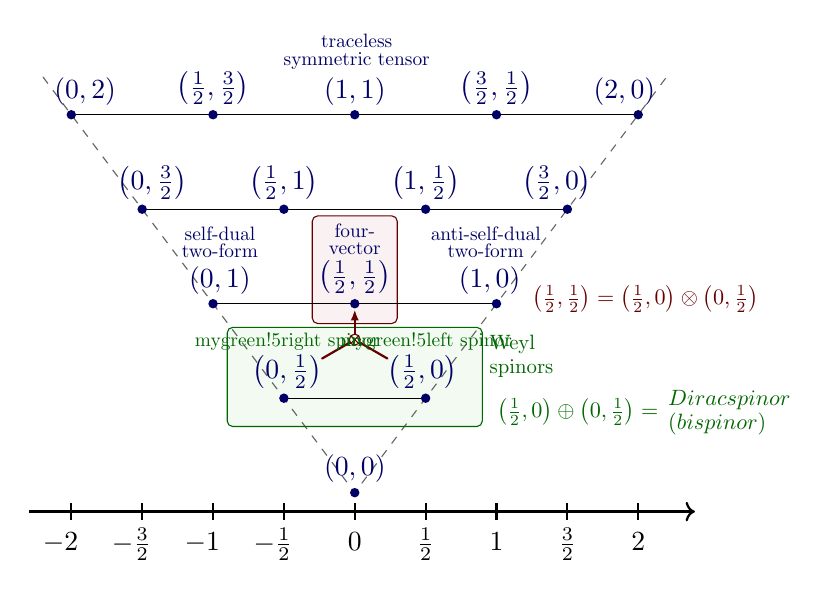
\begin{tikzpicture}[x=1.8cm,y=1.2cm]
\usetikzlibrary{arrows.meta} % to control arrow size
\contourlength{1.2pt}
\newcommand\LP{{\color{mydarkblue}P}} %\Lambda_\mathrm{P}
\newcommand\LT{{\color{mydarkred}T}} %\Lambda_\mathrm{T}
\colorlet{myred}{red!60!black}
\colorlet{myblue}{blue!60!black}
\colorlet{mygreen}{green!60!black}
\colorlet{mydarkblue}{blue!40!black}
\colorlet{mydarkred}{red!40!black}
\colorlet{mydarkgreen}{green!40!black}
\colorlet{mydarkpurple}{blue!50!red!50!black}
\tikzstyle{myarr}=[-{Latex[length=4,width=3]}]


  \def\N{4}      % number of spin states
  \def\r{0.07cm} % radius otimes
  \def\repr#1{   % format simple fraction
    \pgfmathsetmacro{\double}{int(2*#1)}
    \pgfmathsetmacro{\sign}{ifthenelse(#1<0,"-","")}
    \pgfmathparse{int(mod(\double,2))}
    \ifnum0=\pgfmathresult\relax % even
      \pgfmathprintnumber{#1}
    \else % odd
      \sign % sign
      \pgfmathparse{abs(int(\double))}
      \frac{\pgfmathprintnumber{\pgfmathresult}}{2}
    \fi
    \phantom{\sign} % for centered alignment
  }
  
  % AXIS
  \begin{scope}[shift={(0,-0.2)}]
    \draw[->,thick] (-\N/2-0.3,0) -- (\N/2+0.4,0); %node[right=-1] {$S$};
    \foreach \j [evaluate={\x=\j/2; \m=\j/2;}] in {-\N,...,\N}{ % ticks
      \draw[thick] (\x,0.09) --++ (0,-0.18)
        node[below=-1] {\strut$\repr{\m}$}; 
    }
  \end{scope}
  
  % LABELS Dirac spinor
  \draw[dashed,opacity=0.6] (-1.1*\N/2,1.1*\N) -- (0,0) -- (1.1*\N/2,1.1*\N);
  \draw[mydarkgreen,fill=mygreen,fill opacity=0.05,rounded corners=2]
    (-0.9,0.7) rectangle (0.9,1.75)
    node[mydarkgreen,below right,align=left,opacity=1,scale=0.75] {Weyl\\spinors};
  \node[mydarkgreen,scale=0.8,below right] at (0.95,1.2)
    {$\left(\frac{1}{2},0\right)\oplus\left(0,\frac{1}{2}\right)
       = \!\! \begin{array}{l}
           \text{Dirac spinor}\\[-0.5mm]
           \text{(bispinor)}
         \end{array}$};
  %\node[mydarkgreen,scale=0.8,below,align=center] at (1.55,0.68)
  %  {Dirac spinor\\[-3](bispinor)};
  %\node[mydarkgreen,scale=0.8,below,align=center] at (2.58,0.68)
  %  {four-\\[-3]vector};
  %\node[mydarkgreen,scale=0.8,below right] at (1.5,2.2)
  %  {$(1,0)\oplus(0,1) = \text{adjoint}$}; % parity-invariant 2-form field
  
  % LABELS four-vector
  \draw[mydarkred,fill=myred,fill opacity=0.05,rounded corners=2]
    (-0.3,1.79) rectangle (0.3,2.93);
  \node[mydarkred,scale=0.8,right] at (1.2,2.05)
    {$\left(\frac{1}{2},\frac{1}{2}\right) = %\cong
      \left(\frac{1}{2},0\right)\otimes\left(0,\frac{1}{2}\right)$};
  
  % DOTS
  \foreach \j [evaluate={\y=\j;}] in {0,...,\N}{
    \draw (-\j/2,\y) --++ (\j,0);
    \foreach \i [evaluate={
      \m=\i-\j/2;
      \L=\i/2; % left representation
      \R=\j/2-\i/2; % right representation
      \x=\m; % x position
      \myshift=((\i==0||\i==\j)?-2.5*\x:0);
    }] in {0,...,\j}{
      \fill[mydarkblue] (\x,\y) circle (0.06cm);
      \node[mydarkblue,right=\myshift,above]
        %,fill=white,text opacity=1,fill opacity=0.5,inner sep=0.5,outer sep=3
        (P\j-\i) at (\x,\y) {$\left(\repr{\L},\repr{\R}\right)$};
    }
  }
  
  % ARROWS & OTIMES
  \draw[thick,mydarkred,line cap=round]
    (-0.23,1.42) -- (0,1.62) coordinate (A) -- (0.23,1.42);
  \draw[myarr,thick,mydarkred,line cap=round]
    (A) -- (0,1.94);
  \draw[mydarkred,line width=0.4,fill=mygreen!5] % circle
    (A) circle(\r);
  \draw[mydarkred,line width=0.4] % cross
    (A)++(45:\r) --++ (-135:2*\r)
    (A)++(135:\r) --++ (-45:2*\r);
  
  % LABELS
  \node[mydarkgreen,scale=0.7,above=6]
    at (P1-0) {\strut\contour{mygreen!5}{right spinor}};
  \node[mydarkgreen,scale=0.7,right=2,above=6]
    at (P1-1) {\strut\contour{mygreen!5}{left spinor}};
  \node[mydarkblue,scale=0.7,above=8,align=center]
    at (P2-0) {self-dual\\[-3]two-form};
  \node[mydarkblue,scale=0.7,above=8,align=center]
    at (P2-1) {four-\\[-3]vector};
  \node[mydarkblue,scale=0.7,left=2,above=8,align=center]
    at (P2-2) {anti-self-dual\\[-3]two-form};
  \node[mydarkblue,scale=0.7,right=1,above=8,align=center]
    at (P4-2) {traceless\\[-3]symmetric tensor};
  
\end{tikzpicture}




\end{itemize}



\end{document}